%! TEX program = xelatex
% {{{ PREAMBLE
\documentclass[10pt,aspectratio=169]{beamer}

\graphicspath{{img/}{../img/}}
\usepackage[T1]{fontenc}
\usepackage[english]{babel}

\usepackage{microtype}
\usepackage{booktabs}
\usepackage{multirow}
  \newcommand{\mr}[2]{\multirow{#1}{*}{#2}}
\usepackage{multicol}
  \newcommand{\mc}[2]{\multicolumn{#1}{c}{#2}}
\usepackage{makecell}
\usepackage{relsize}

\usepackage{enumerate}
\usepackage{listings}
\usepackage{xcolor}
\usepackage{tikz}

% {{{ colors
\setbeamercolor{background canvas}{bg=white}
\newcommand{\mlbrown}[1]{\textcolor{mLightBrown}{#1}}
\newcommand{\mdbrown}[1]{\textcolor{mDarkBrown}{#1}}
\newcommand{\mlgreen}[1]{\textcolor{mLightGreen}{#1}}
\newcommand{\mdteal}[1]{\textcolor{mDarkTeal}{#1}}
% Available aliases: \<color>{<text>}
%
%   tlblue tlred tlpurple tlgreen tlbrown
%   tdblue tdred tdpurple tdgreen tdbrown
%
\usepackage{pgfplots}
\usepackage{pgfplotsthemetol}
\newcommand{\tlblue}[1]{\textcolor{TolLightBlue}{#1}}
\newcommand{\tdblue}[1]{\textcolor{TolDarkBlue}{#1}}
\newcommand{\tlred}[1]{\textcolor{TolLightRed}{#1}}
\newcommand{\tdred}[1]{\textcolor{TolDarkRed}{#1}}
\newcommand{\tlpurple}[1]{\textcolor{TolLightPurple}{#1}}
\newcommand{\tdpurple}[1]{\textcolor{TolDarkPurple}{#1}}
\newcommand{\tlpink}[1]{\textcolor{TolLightPink}{#1}}
\newcommand{\tdpink}[1]{\textcolor{TolDarkPink}{#1}}
\newcommand{\tlgreen}[1]{\textcolor{TolLightGreen}{#1}}
\newcommand{\tdgreen}[1]{\textcolor{TolDarkGreen}{#1}}
\newcommand{\tlbrown}[1]{\textcolor{TolLightBrown}{#1}}
\newcommand{\tdbrown}[1]{\textcolor{TolDarkBrown}{#1}}
% }}}

% check marks
\usepackage{pifont}
\newcommand{\cmark}{\textcolor{mLightGreen}{\ding{51}}}
\newcommand{\xmark}{\textcolor{mLightBrown}{\ding{55}}}

% math
\usepackage{amsmath}
\renewcommand{\epsilon}{\varepsilon}
\renewcommand{\theta}{\vartheta}
\renewcommand{\rho}{\varrho}
\renewcommand{\phi}{\varphi}
\usepackage{amsfonts}
\usepackage[mathrm=sym]{unicode-math}
\setmathfont{Fira Math}

%!TEX root = ../main.tex

\newcommand{\n}           {$\upnu$}
\newcommand{\x}           {$\upchi$}
\renewcommand{\b}         {$\upbeta$}
\newcommand{\g}           {$\upgamma$}
\renewcommand{\a}         {$\upalpha$}
\newcommand{\NAZ}         {$\mathcal{N}(A,Z)$}
\newcommand{\cpt}         {$CPT$}
\newcommand{\aofM}        {{\mathring{a}_\text{of}^{(3)}}}
\newcommand{\aof}         {$\aofM$}
\newcommand{\aofooM}      {{{(a_\text{of}^{(3)})}_{00}}}
\newcommand{\aofoo}       {$\aofooM$}

\newcommand{\fillme}   [1]{\textcolor{red}{\texttt{#1}}}
\newcommand{\reg}         {\textsuperscript{\textregistered}}

% data sets
\newcommand{\m}        [1]{\texttt{#1}}
\newcommand{\bege}        {\textsc{BEGe}}
\newcommand{\scoax}       {\textsc{SemiCoax}}
\newcommand{\icoax}       {\textsc{InvCoax}}
\newcommand{\GD}       [1]{\m{GD#1}}
\newcommand{\ANG}      [1]{\m{ANG#1}}
\newcommand{\GTF}      [1]{\m{GTF#1}}
\newcommand{\RG}       [1]{\m{RG#1}}
\newcommand{\IC}       [1]{\m{IC#1}}
\newcommand{\pplus}       {p$^+$}
\newcommand{\nplus}       {n$^+$}

% global model
\newcommand{\Mone}        {\m{M1}}
\newcommand{\Mtwo}        {\m{M2}}
\newcommand{\enrBEGeII}   {\m{M1-BEGe}}
\newcommand{\enrCoaxII}   {\m{M1-SemiCoax}}
\newcommand{\enrGeII}     {\m{M2-AllEnr}}
\newcommand{\enrBEGeIIp}  {\m{M1-BEGe\textsuperscript{+}}}
\newcommand{\enrSCoaxIIp} {\m{M1-SemiCoax\textsuperscript{+}}}
\newcommand{\enrICoaxIIp} {\m{M1-InvCoax\textsuperscript{+}}}
\newcommand{\enrGeIIp}    {\m{M2-AllEnr\textsuperscript{+}}}
% K model
\newcommand{\Mokvn}{\m{M1-K40}}
\newcommand{\Mtkvn}{\m{M2-K40}}
\newcommand{\Mokvz}{\m{M1-K42}}
\newcommand{\Mtkvz}{\m{M2-K42}}
\newcommand{\MoSBon}{\m{M1-SB1}}
\newcommand{\MtSBon}{\m{M2-SB1}}
\newcommand{\MoSBtw}{\m{M1-SB2}}
\newcommand{\MtSBtw}{\m{M2-SB2}}
\newcommand{\MoSBth}{\m{M1-SB3}}
\newcommand{\MtSBth}{\m{M2-SB3}}

\newcommand{\annmse}         {ANN$_\text{MSE}$}
\newcommand{\deltae}         {$\delta{E}$}
\newcommand{\aoe}            {$A/E$}
\newcommand{\measurementM}[3]{{#1}\substack{+#2 \\ -#3}}
\newcommand{\measurement} [3]{$\measurementM{#1}{#2}{#3}$}
\newcommand{\stat}        [1]{{#1}_\text{stat}}
\newcommand{\syst}        [1]{{#1}_\text{sys}}
\newcommand{\pvalue}         {$p$-value}

% units
\newcommand{\ctsper}      {cts/(keV$\cdot$kg$\cdot$yr)}
\newcommand{\powctsper}[1]{{$10^{#1}$~cts/(keV$\cdot$kg$\cdot$yr)}}
\newcommand{\pIbi}        {{$1.2\cdot10^{-2}$~cts/(keV$\cdot$kg$\cdot$yr)}}
\newcommand{\pIIbi}       {{$10^{-3}$~cts/(keV$\cdot$kg$\cdot$yr)}}
\newcommand{\kgy}         {{kg$\cdot$yr}}
\newcommand{\kgyr}        {{kg$\cdot$yr}}
\newcommand{\kevkgyr}     {{keV$\cdot$kg$\cdot$yr}}
\newcommand{\mubq}        {{$\upmu$Bq}}
\newcommand{\mum}         {{$\upmu$m}}
\newcommand{\mus}         {{$\upmu$s}}
%\newcommand{\mubqperkg}   {{$\frac{\upmu\mathrm{Bq}}{\mathrm{kg}}$}}
\newcommand{\mubqperkg}   {{${\upmu\mathrm{Bq}}/{\mathrm{kg}}$}}
\newcommand{\powtenyr} [1]{$10^{#1}$~yr}

% dbd
\newcommand{\qbbM}        {Q_{\upbeta\upbeta}}
\newcommand{\qbb}         {$\qbbM$}
\newcommand{\thalfzeroM}  {{T^{0\upnu}_{1/2}}}
\newcommand{\thalftwoM}   {{T^{2\upnu}_{1/2}}}
\newcommand{\thalfzero}   {$\thalfzeroM$}
\newcommand{\thalftwo}    {$\thalftwoM$}
\newcommand{\thalfmajo}   {{${T^{0\upnu\upchi(\upchi)}_{1/2}}$}}
\newcommand{\thalfzx}     {{${T^{0\upnu\upchi}_{1/2}}$}}
\newcommand{\thalfzxx}    {{${T^{0\upnu\upchi\upchi}_{1/2}}$}}
\newcommand{\nmez}        {$\mathcal{M}^{0\upnu}$}
\newcommand{\nmet}        {$\mathcal{M}^{2\upnu}$}
\newcommand{\nmemajo}     {$\mathcal{M}^{0\upnu\upchi(\upchi)}$}
\newcommand{\psfz}        {$G^{0\upnu}$}
\newcommand{\psft}        {$G^{2\upnu}$}
\newcommand{\psfmajo}     {$G^{0\upnu\upchi(\upchi)}$}
\newcommand{\mbb}         {$\langle{m_{\upbeta\upbeta}}\rangle$}
\newcommand{\mb}          {$m_{\upbeta}$}
\newcommand{\onbbM}       {{0\upnu\upbeta\upbeta}}
\newcommand{\onbb}        {$\onbbM$}
\newcommand{\onbbp}       {$0\upnu\upbeta^+\upbeta^+$}
\newcommand{\onbbm}       {$0\upnu\upbeta^-\upbeta^-$}
\newcommand{\nnbb}        {$2\upnu\upbeta\upbeta$}
\newcommand{\nnbbp}       {$2\upnu\upbeta^+\upbeta^+$}
\newcommand{\nnbbm}       {$2\upnu\upbeta^-\upbeta^-$}
\newcommand{\onbbx}       {$0\upnu\upbeta\upbeta\upchi$}
\newcommand{\onbbxx}      {$0\upnu\upbeta\upbeta\upchi\upchi$}
\newcommand{\nnbblv}      {$2\upnu\upbeta\upbeta_\text{LV}$}
\newcommand{\onecec}      {$0\upnu\text{ECEC}$}
\newcommand{\nnecec}      {$2\upnu\text{ECEC}$}
\newcommand{\tlive}       {\mbox{$t_{live}$}}
\newcommand{\flive}       {\mbox{$f_{live}$}}
\newcommand{\fge}         {\mbox{$f_{Ge}$}}
\newcommand{\fgesix}      {\mbox{$f_{76}$}}
\newcommand{\fgesixi}     {\mbox{$f_{76,i}$}}
\newcommand{\actmass}     {\mbox{$M_{act}$}}
\newcommand{\ssmass}      {\mbox{$M_{76}$}}
\newcommand{\factmass}    {\mbox{$f_{av}$}}
\newcommand{\factmassi}   {\mbox{$f_{av,i}$}}
\newcommand{\factvol}     {\mbox{$f_{av}$}}
\newcommand{\factvoli}    {\mbox{$f_{av,i}$}}
\newcommand{\subssix}     {\mbox{$_{76}$}}
\newcommand{\subssixi}    {\mbox{$_{76,i}$}}
\newcommand{\subav}       {\mbox{$_{av}$}}
\newcommand{\subavi}      {\mbox{$_{av,i}$}}

\newcommand{\gerdafinallimit}{$\thalfzeroM = 1.8 \cdot 10^{26}$~yr}
\newcommand{\gexpophasetwo}{60.1~\kgyr}
\newcommand{\gexpophasetwobkg}{61.4~\kgyr}
\newcommand{\gexpophasetwop}{43.6~\kgyr}
\newcommand{\gexpophasetwopbkg}{44.1~\kgyr}
\newcommand{\gexpobkg}{105.5~\kgyr}
\newcommand{\gexpo}{103.7~\kgyr}

% experiments and equipment
\newcommand{\gerda}       {\textsc{Gerda}}
\newcommand{\phaseone}    {Phase~I}
\newcommand{\phasetwo}    {Phase~II}
\newcommand{\phasetwop}   {Phase~II$^+$}
\newcommand{\gerdatwo}    {\gerda\ Phase~II}
\newcommand{\LArGe}       {\textsc{LArGe}}
\newcommand{\majorana}    {\textsc{Majorana}}
\newcommand{\majoranademo}{\textsc{Majorana Demonstrator}}
\newcommand{\igex}        {\textsc{Igex}}
\newcommand{\hdm}         {\textsc{HdM}}
% code
\newcommand{\geant}       {\textsc{Geant4}}
\newcommand{\GEANT}       {\textsc{\mbox{{Geant}}}}
\newcommand{\rootv}       {\textsc{Root}}
\newcommand{\CERN}        {{\mbox{\textsc{Cern}}}}
\newcommand{\mage}        {\textsc{MaGe}}
\newcommand{\gelatio}     {\textsc{Gelatio}}
\newcommand{\mgdo}        {\mbox{MGDO}}
\newcommand{\tier}        {\textsc{Tier}}
\newcommand{\decayzero}   {\textsc{Decay0}}
% isotopes
\newcommand{\gesix}       {$^{76}$Ge}
\newcommand{\geseven}     {$^{77}$Ge}
\newcommand{\gefour}      {$^{74}$Ge}
\newcommand{\gethree}     {$^{73}$Ge}
\newcommand{\gess}        {$^{76}$Ge}
\newcommand{\gesf}        {$^{74}$Ge}
\newcommand{\geenr}       {$^{\rm enr}$Ge}
\newcommand{\genat}       {$^{\rm nat}$Ge}
\newcommand{\gedep}       {$^{\rm dep}$Ge}
\newcommand{\geox}        {GeO$_2$}
\newcommand{\enrgecoax}   {$^{\rm enr}$Ge-coax}
\newcommand{\nuc}      [2]{$^{#2}${#1}}
\newcommand{\kvn}         {$^{40}$K}
\newcommand{\kvz}         {$^{42}$K}
\newcommand{\Am}          {$^{241}$Am}
\let\Rn\undefined\newcommand{\Rn}{$^{222}$Rn}
\newcommand{\Ra}          {$^{226}$Ra}
\newcommand{\Po}          {$^{210}$Po}
\newcommand{\Arh}         {$^{42}$Ar}
\newcommand{\Arl}         {$^{39}$Ar}
\newcommand{\Kr}          {$^{85}$Kr}
\newcommand{\Xe}          {$^{133}$Xe}
\newcommand{\Ba}          {$^{133}$Ba}
\newcommand{\Bil}         {$^{212}$Bi}
\newcommand{\Bih}         {$^{214}$Bi}
\newcommand{\Yb}          {$^{176}$Yb}
\newcommand{\Fe}          {$^{55}$Fe}
\newcommand{\Thh}         {$^{232}$Th}
\newcommand{\Th}          {$^{228}$Th}
\newcommand{\Tl}          {$^{208}$Tl}
\newcommand{\Ul}          {$^{235}$U}
\newcommand{\Uh}          {$^{238}$U}
\newcommand{\Be}          {$^7$Be}
\newcommand{\Co}          {$^{60}$Co}
\newcommand{\Ac}          {$^{228}$Ac}
\newcommand{\Pbl}         {$^{210}$Pb}
\newcommand{\Pbh}         {$^{214}$Pb}
\newcommand{\Pa}          {$^{234\text{m}}$Pa}
\newcommand{\Zn}          {$^{65}$Zn}

\newcommand{\expoM}   {\mathcal{E}}
\newcommand{\expo}    {$\expoM$}


\newcommand{\mytitle}{Search for new physics with \texorpdfstring{\nnbb}{2νββ} decay in \gerda}
\newcommand{\people}{L.~Pertoldi}
\institute{Universit\`a degli Studi di Padova / INFN Padova}
\newcommand{\mydate}{23 Feb 2021}
\newcommand{\place}{\textit{\gerda\ clean room}}

% links
\definecolor{TolDARKBlue}{HTML}{3973AC}
\hypersetup{%
  pdfauthor = {Luigi Pertoldi},
  pdftitle = {Search for new physics with 2νββ in GERDA data (slides)},
  pdfkeywords = {physics, neutrino, double-beta},
  pdfproducer = {XeLaTeX with hyperref},
  pdfcreator = {XeLaTeX},
  colorlinks = true,
  urlcolor = TolDARKBlue,
  linkcolor = mDarkTeal
}
\renewcommand\UrlFont{\color{TolDARKBlue}}
\newcommand{\doi}[1]{\href{https://doi.org/#1}{\smaller\ttfamily #1}}
\newcommand{\arxiv}[1]{\href{https://arxiv.org/abs/#1}{\smaller\ttfamily arXiv:#1}}
\newcommand{\github}[1]{
\includegraphics[height=6pt]{logos/gihub-logo.png}:~\href{https://github.com/#1}{#1}}

% metropolis theme options
\usetheme[numbering=fraction,block=fill]{metropolis}
\setbeamertemplate{frame footer}{\emph{\mytitle} $\bullet$ \people\ $\bullet$ Ph.D.~defense $\bullet$ \mydate}
\title{\mytitle}
% \subtitle{Ph.D.~Defense}
\titlegraphic{%
  \vspace{4.2cm}%
    \begin{minipage}[c]{\textwidth}
      \hfill%
      \raisebox{-0.5\height}{
\includegraphics[height=1.7cm]{img/logos/unipd-logo.pdf}}%
      \hspace{0.3cm}%
      \raisebox{-0.5\height}{
\includegraphics[height=1.7cm]{img/logos/infn-logo.pdf}}%
      \hspace{0.3cm}%
      \raisebox{-0.5\height}{
\includegraphics[height=1.7cm]{img/logos/gerda-logo.png}}%
    \end{minipage}
}
\date{\place\ \sep\ \mydate}
\author{\people}

% {{{ customization
\usepackage{appendixnumberbeamer}
\setbeamercovered{dynamic}
% for heavier glyphs
\setsansfont[BoldFont={Fira Sans SemiBold}]{Fira Sans Book}
\setmonofont{Fira Code}[Contextuals=Alternate, Scale=0.8]
% usage: \begin{simpleblock} ... \end{simpleblock}
\usepackage[most]{tcolorbox}
\newtcolorbox{simpleblock}{
%  enhanced,  % does not work with tikz/external
  boxsep=0.25ex,
%  arc=1.25ex,
  arc=0ex,
  opacityframe=.6,
  opacityback=.6,
  colback=bg!80!fg,
  coltext=mDarkTeal,
  colframe=white,
  boxrule=0pt,
}
% }}}

\newcommand{\arrow}{$\longmapsto$}
\newcommand{\sep}{$\bullet$}

\newcommand\blfootnote[1]{%
  \begingroup
  \renewcommand\thefootnote{}\footnote{#1}%
  \addtocounter{footnote}{-1}%
  \endgroup
}

% }}}
% \includeonlyframes{compile}
\begin{document}
\maketitle
\begin{frame}{About me}
  \begin{columns}
    \begin{column}{0.45\textwidth}\setlength{\parskip}{5pt}%
      \vspace*{1cm} \\
      \textbf{Currently:} postdoc at \emph{TU M\"unchen}, \gerda/LEGEND group
      \begin{itemize}
        \item \href{https://gipert.github.io}{gipert.github.io}
        \item \href{https://orcid.org/0000-0002-0467-2571}{orcid.org/0000-0002-0467-2571}
        \item \href{https://inspirehep.net/authors/1667599}{inspirehep.net/authors/1667599}
      \end{itemize}

      \textbf{Topic:} \gerda\ simulation \& background studies (task group leader)

      \vspace*{0.5cm}
      \footnotesize
      \textbf{[slides]} \href{https://l.infn.it/pertoldi-phd-sl}{l.infn.it/pertoldi-phd-sl} \\
      \textbf{[thesis]} \href{https://l.infn.it/pertoldi-phd-th}{l.infn.it/pertoldi-phd-th}
    \end{column}
    \begin{column}{0.55\textwidth}
      \vspace*{5mm}
      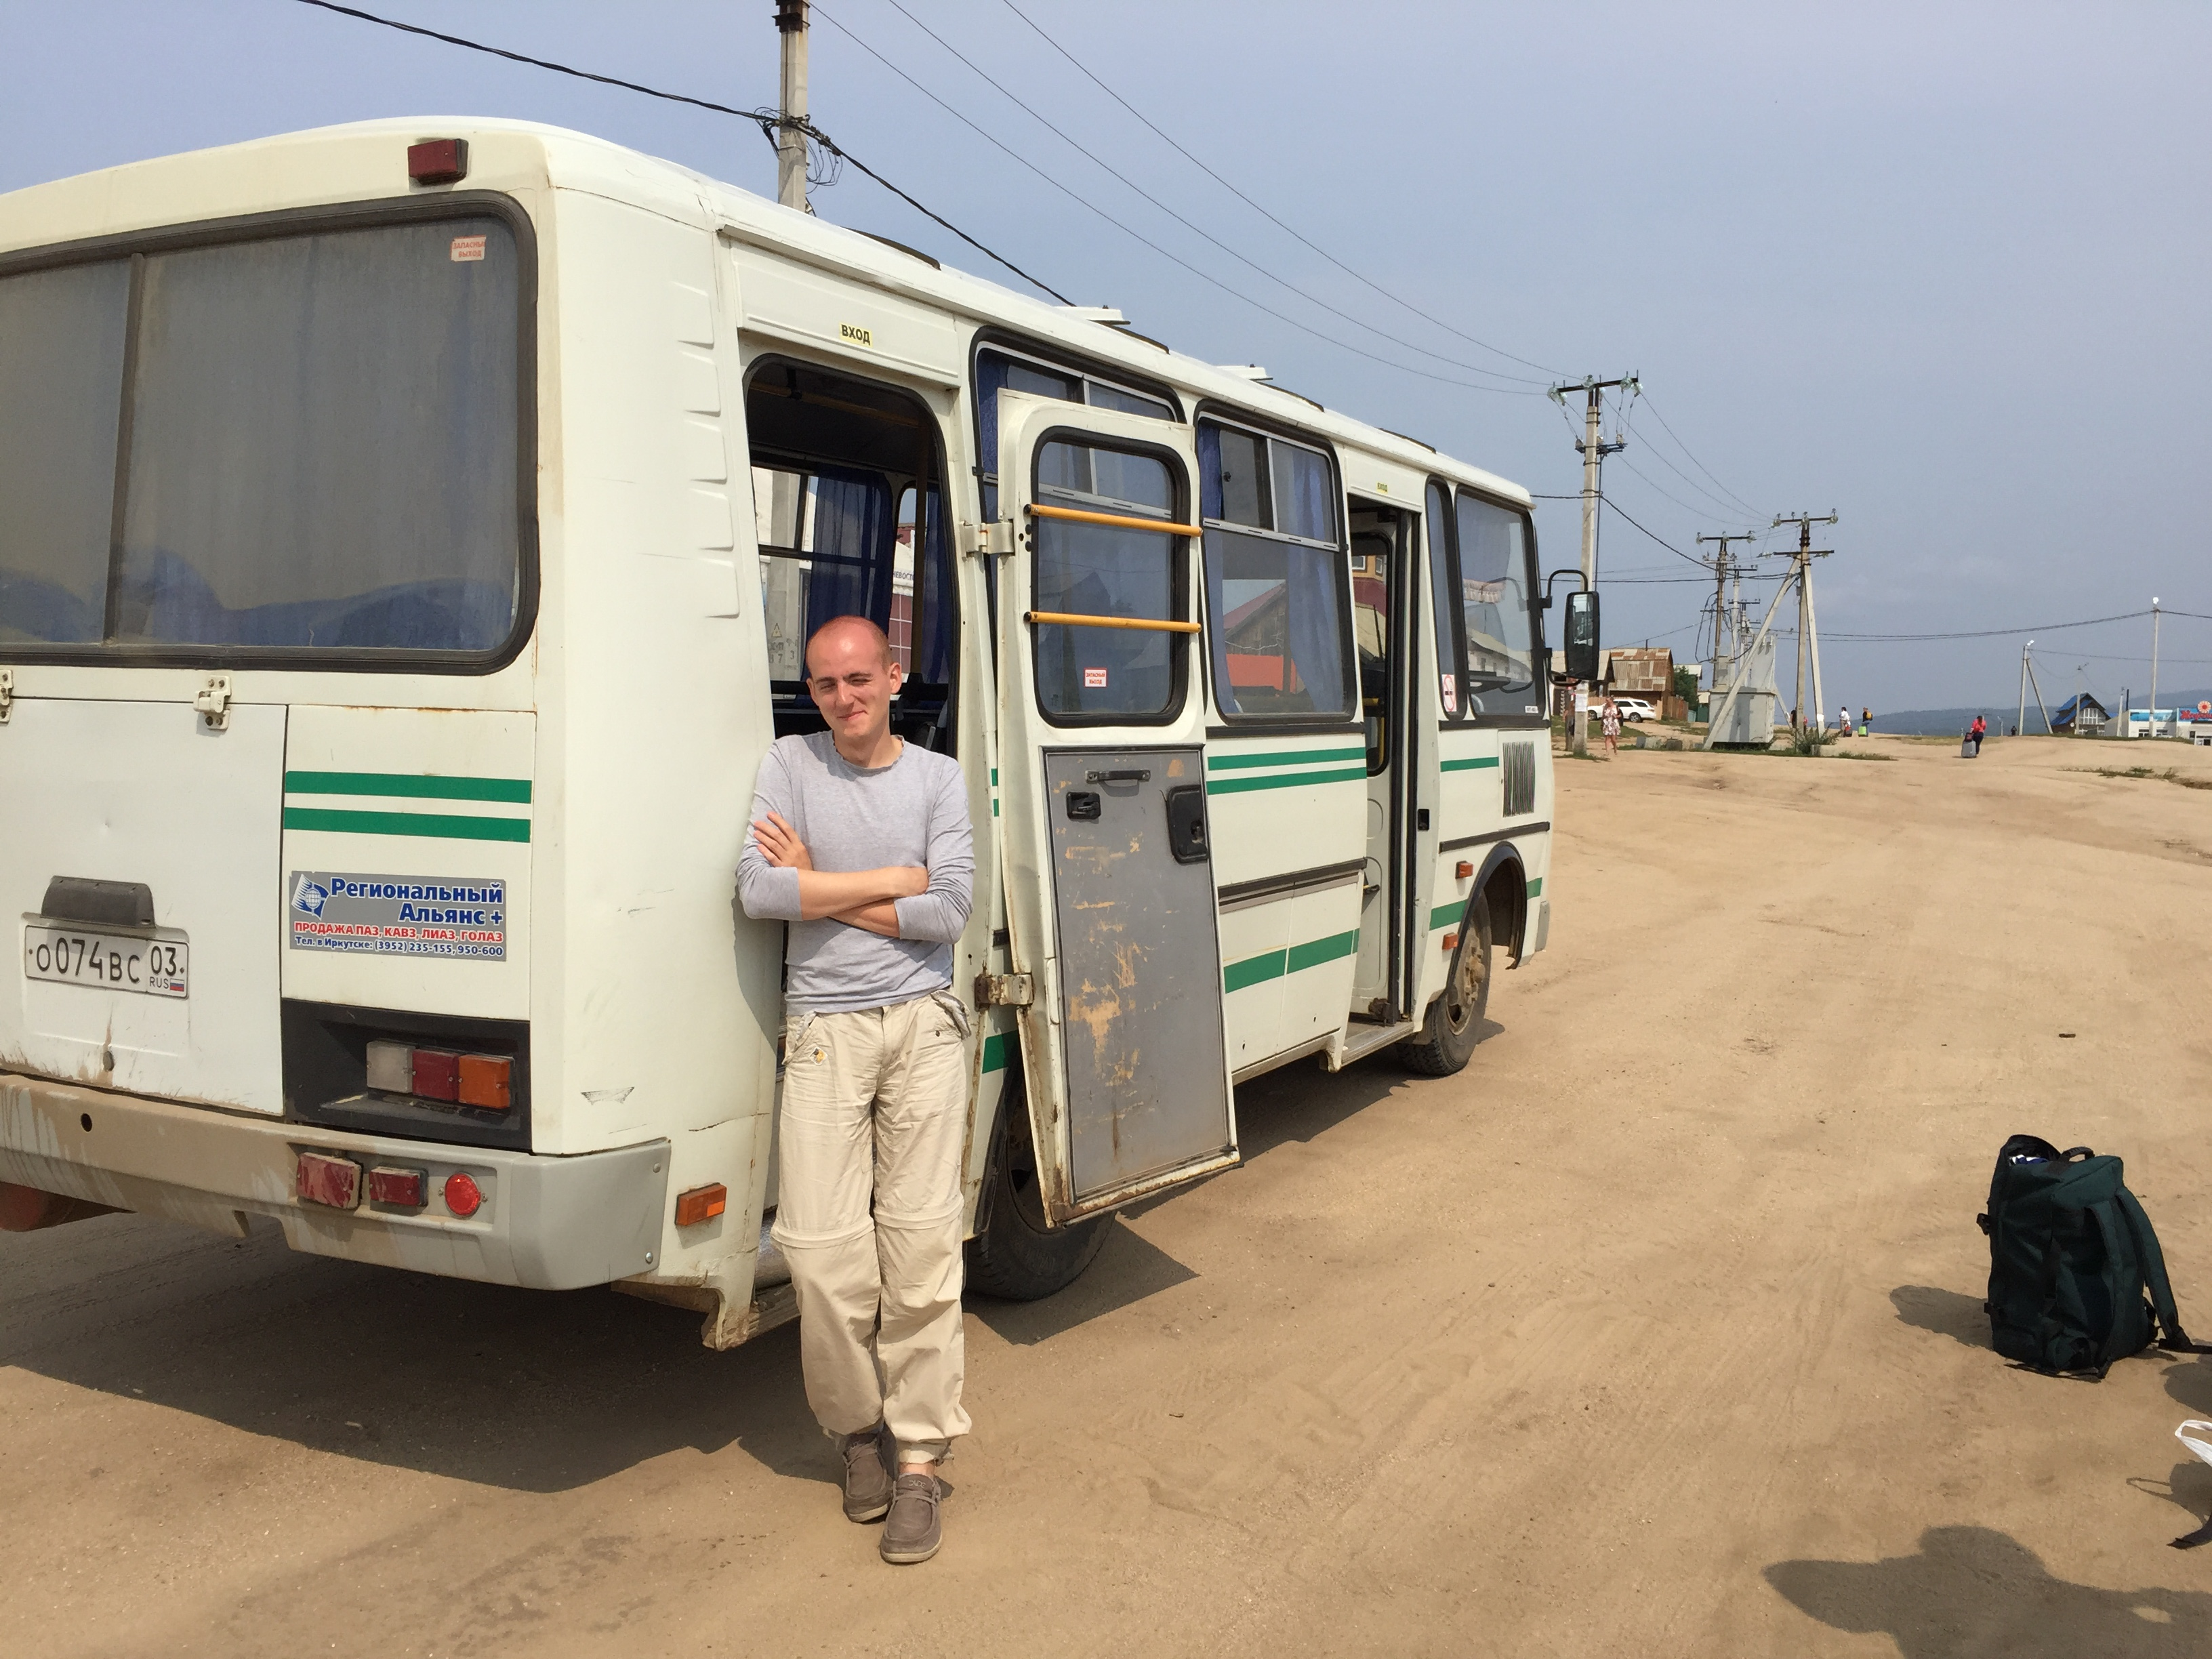
\includegraphics[trim=0 0 0 0,clip,width=\columnwidth]{me-siberia.jpg}
    \end{column}
  \end{columns}
\end{frame}
\begin{frame}{Outline}
  \begin{enumerate}
    \item Why studying \alert{double-beta} decay?
      \begin{itemize}
        \item Rare physics, origins of the Universe, Majorana neutrino, Standard Model probe
      \end{itemize}
    \item \alert{\gerda} --- science goal and experimental design
      \begin{itemize}
        \item Underground \gesix\ detectors, background mitigation techniques, latest results
      \end{itemize}
    \item The \gerda\ \alert{background model} before analysis cuts
      \begin{itemize}
        \item Monte Carlo simulations, background expectations, statistical techniques
      \end{itemize}
    \item The \gerda\ background model \alert{after the LAr veto cut}
      \begin{itemize}
        \item LAr veto system, optical Monte Carlo simulations, LAr veto calibration data
      \end{itemize}
    \item Precision analysis of the \alert{\nnbb\ event distribution}
    \begin{itemize}
      \item Bayesian-frequentist analysis, \nnbb\ half-life measurement, new-physics, systematics
    \end{itemize}
  \end{enumerate}
\end{frame}
\section{Double-beta decay}
\begin{frame}{Two-neutrino double-beta decay}
  \begin{center}
    \begin{tikzpicture}[font=\small]
      \node at (2.0,0) {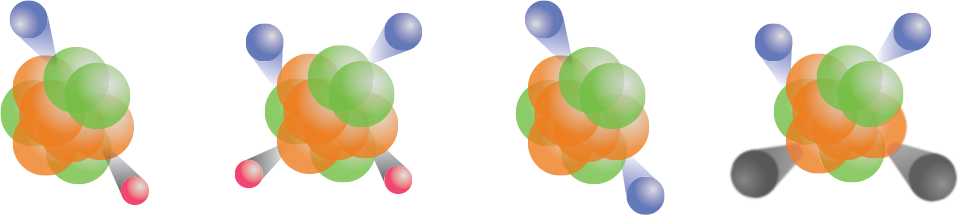
\includegraphics[height=2.8cm]{plots/theory/bb-artist-newphy.png}};

      \node[align=center] at (-3.4,-1.9) {\scshape $\upbeta$ decay};
      \node[align=center] at ( 0.2,-1.9) {\scshape double-$\upbeta$ decay};
      \node[align=center] at ( 3.4,-1.9) {\scshape neutrinoless \\ \scshape double-$\upbeta$ decay};
      \node[align=center] at ( 6.8,-1.9) {\scshape Majoron \\ \scshape emission};

      \node at (-4.2, 1.5) {$e^-$};
      \node at (-2.1,-1.1) {\footnotesize $\overline{\upnu}_e$};

      \node at (-1.2, 1.1) {$e^-$};
      \node at ( 1.4, 1.2) {$e^-$};
      \node at ( 1.4,-1.0) {\footnotesize $\overline{\upnu}_e$};
      \node at (-1.4,-0.9) {\footnotesize $\overline{\upnu}_e$};

      \node at ( 3.2, 1.5) {$e^-$};
      \node at ( 4.6,-1.2) {$e^-$};

      \node at ( 5.6, 1.2) {$e^-$};
      \node at ( 8.1, 1.2) {$e^-$};
      \node at ( 5.2,-1.2) {$\chi$};
      \node at ( 8.3,-1.2) {$\chi$};

      \draw[draw=none,fill=white,opacity=0.7] (2.0,-2.3) rectangle (8.4,1.8);
    \end{tikzpicture}
  \end{center}
\end{frame}
\begin{frame}{Neutrinoless double-beta decay}
  \begin{center}
    \begin{tikzpicture}[font=\small]
      \node at (2.0,0) {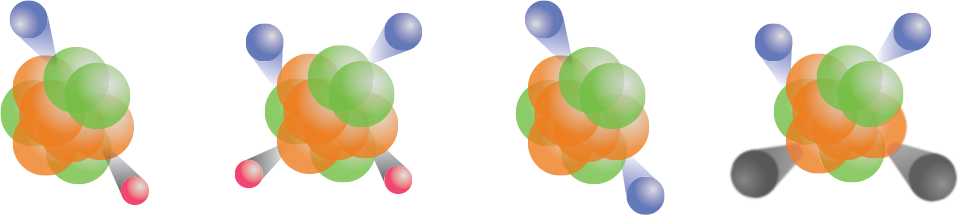
\includegraphics[height=2.8cm]{plots/theory/bb-artist-newphy.png}};

      \node[align=center] at (-3.4,-1.9) {\scshape $\upbeta$ decay};
      \node[align=center] at ( 0.2,-1.9) {\scshape double-$\upbeta$ decay};
      \node[align=center] at ( 3.4,-1.9) {\scshape neutrinoless \\ \scshape double-$\upbeta$ decay};
      \node[align=center] at ( 6.8,-1.9) {\scshape Majoron \\ \scshape emission};

      \node at (-4.2, 1.5) {$e^-$};
      \node at (-2.1,-1.1) {\footnotesize $\overline{\upnu}_e$};

      \node at (-1.2, 1.1) {$e^-$};
      \node at ( 1.4, 1.2) {$e^-$};
      \node at ( 1.4,-1.0) {\footnotesize $\overline{\upnu}_e$};
      \node at (-1.4,-0.9) {\footnotesize $\overline{\upnu}_e$};

      \node at ( 3.2, 1.5) {$e^-$};
      \node at ( 4.6,-1.2) {$e^-$};

      \node at ( 5.6, 1.2) {$e^-$};
      \node at ( 8.1, 1.2) {$e^-$};
      \node at ( 5.2,-1.2) {$\chi$};
      \node at ( 8.3,-1.2) {$\chi$};

      \draw[draw=none,fill=white,opacity=0.7] (-4.4,-2.3) rectangle (2.0,1.8);
      \draw[draw=none,fill=white,opacity=0.7] ( 5.0,-2.3) rectangle (8.4,1.8);
    \end{tikzpicture}
  \end{center}
\end{frame}
\begin{frame}{Why searching for neutrinoless double-$\beta$ decay?}
  Huge literature production\footnote{%
    100+ papers per year with ``\onbb'' in the title
    \href{https://inspirehep.net/literature?sort=mostrecent&size=25&page=1&q=find\%20t\%20\%CE\%B2\%CE\%B2\%20or\%20double-beta\%20or\%20double\%20beta\%20or\%20double\%20\%CE\%B2\%20or\%20double-\%CE\%B2\%20or\%200\%CE\%BD\%CE\%B2\%CE\%B2&ui-citation-summary=true}{[INSPIRE-HEP statistics]}
  }
  \begin{itemize}
    \item \onbb\ observation $\Rightarrow$ \alert{Majorana neutrino} and \alert{Lepton number violation}
    \item Lepton number $\longleftrightarrow$ Barion number \arrow\
      \alert{new physics}, \alert{baryogenesis?}
    \item Access to fundamental parameters, shared or not with other
      physics searches
    \item \alert{standard interpretation}: \emph{the neutrino that mediates
      \onbb\ is the one that oscillates and the Standard Model is an effective
      theory of some GUT} (seesaw mechanism)
    \begin{itemize}
      \item Majorana effective mass \mbb:
        $(T^{0\nu}_{1/2})^{-1}=G_{0\nu} |\mathcal{M}_{0\nu}|^2 \alert{m_{\beta\beta}}^2$
        \arrow\ PMNS and neutrino mass
    \end{itemize}
  \item countless non-standard interpretations\footnote{See e.g.~\href{https://doi.org/10.1088/1367-2630/17/11/115010}{\emph{New J.~Phys.}~17 (2015) 11, 115010}}
  \end{itemize}
\end{frame}
\begin{frame}{Neutrinoless double-beta decay: signature}
  \begin{columns}
    \begin{column}{0.5\textwidth}
      \begin{center}
        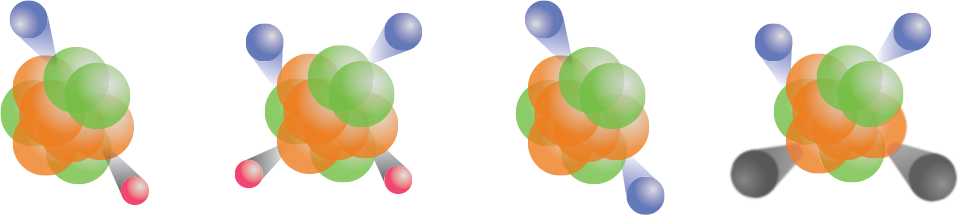
\includegraphics[width=2.5cm,angle=-90,clip,trim=200 0 500 0]{plots/theory/bb-artist-newphy.png}
      \end{center}

      Most experiments measure the \alert{total energy of the two emitted
      electrons}

      \vspace*{16pt}
      \arrow\ \emph{necessary and sufficient} for discovery
    \end{column}
    \begin{column}{0.5\textwidth}
      \begin{center}
        \includegraphics{plots/theory/bb-spectra.pdf}
      \end{center}
    \end{column}
  \end{columns}
\end{frame}
\begin{frame}{Double-beta decay and Majoron emission}
  \begin{center}
    \begin{tikzpicture}[font=\small]
      \node at (2.0,0) {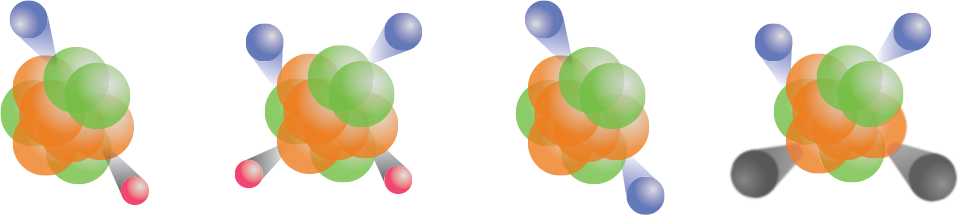
\includegraphics[height=2.8cm]{plots/theory/bb-artist-newphy.png}};

      \node[align=center] at (-3.4,-1.9) {\scshape $\upbeta$ decay};
      \node[align=center] at ( 0.2,-1.9) {\scshape double-$\upbeta$ decay};
      \node[align=center] at ( 3.4,-1.9) {\scshape neutrinoless \\ \scshape double-$\upbeta$ decay};
      \node[align=center] at ( 6.8,-1.9) {\scshape Majoron \\ \scshape emission};

      \node at (-4.2, 1.5) {$e^-$};
      \node at (-2.1,-1.1) {\footnotesize $\overline{\upnu}_e$};

      \node at (-1.2, 1.1) {$e^-$};
      \node at ( 1.4, 1.2) {$e^-$};
      \node at ( 1.4,-1.0) {\footnotesize $\overline{\upnu}_e$};
      \node at (-1.4,-0.9) {\footnotesize $\overline{\upnu}_e$};

      \node at ( 3.2, 1.5) {$e^-$};
      \node at ( 4.6,-1.2) {$e^-$};

      \node at ( 5.6, 1.2) {$e^-$};
      \node at ( 8.1, 1.2) {$e^-$};
      \node at ( 5.2,-1.2) {$\chi$};
      \node at ( 8.3,-1.2) {$\chi$};

      \draw[draw=none,fill=white,opacity=0.7] (-4.4,-2.3) rectangle (5.0,1.8);
    \end{tikzpicture}
  \end{center}
\end{frame}
\begin{frame}{Neutrinoless double-beta decay with Majoron emission}
  \begin{columns}
    \begin{column}{0.5\textwidth}
      \begin{itemize}
        \item The \alert{Majoron ($\chi$)} is an hypothetical (here massless)
          particle
        \item Many models for \onbb\ with one or more emitted Majorons
      \end{itemize}
      \begin{simpleblock}
        \[
          G_\alpha^{0\upnu\upchi(\upchi)} \sim {(Q_{\upbeta\upbeta} - K)}^n
        \]
      \end{simpleblock}
    \end{column}
    \begin{column}{0.5\textwidth}
      \begin{center}
        \includegraphics{plots/theory/majorons-spectra.pdf}
      \end{center}
    \end{column}
  \end{columns}
\end{frame}
\section{The \gerda\ experiment}
\begin{frame}{\texorpdfstring{\onbb}{0νββ} experimental searches}
  \begin{columns}
    \begin{column}{0.5\textwidth}
      \begin{itemize}
        \item \textbf{Bolometers} CUORE (\nuc{Te}{130}), CUPID, \textsc{AMoRE}
        \item \textbf{Time projection chambers (\nuc{Xe}{136})} EXO, NEXT, \textsc{PandaX}
        \item \textbf{Scintillators} \kamlandzen\ (\nuc{Xe}{136}), SNO+, CANDLES
        \item \textbf{Tracking calorimeters} NEMO, \textsc{SuperNEMO}
      \end{itemize}
    \end{column}
    \begin{column}{0.5\textwidth}
      \begin{alertblock}{Semiconductors: \gerda, \majoranademo, LEGEND (\gesix)}
        \begin{itemize}\small
          \item[\cmark] \gesix-enriched detector technology maturity
          \item[\cmark] Excellent energy resolution
          \item[\xmark] Production cost, Low Q-value
        \end{itemize}
      \end{alertblock}
      \begin{center}
        \includegraphics[width=0.9\columnwidth]{setup/gedet-showcase.png}
      \end{center}
    \end{column}
  \end{columns}
\end{frame}
\begin{frame}{More than 50 years of \gesix\ \texorpdfstring{\onbb}{0νββ} searches}
  \begin{center}
    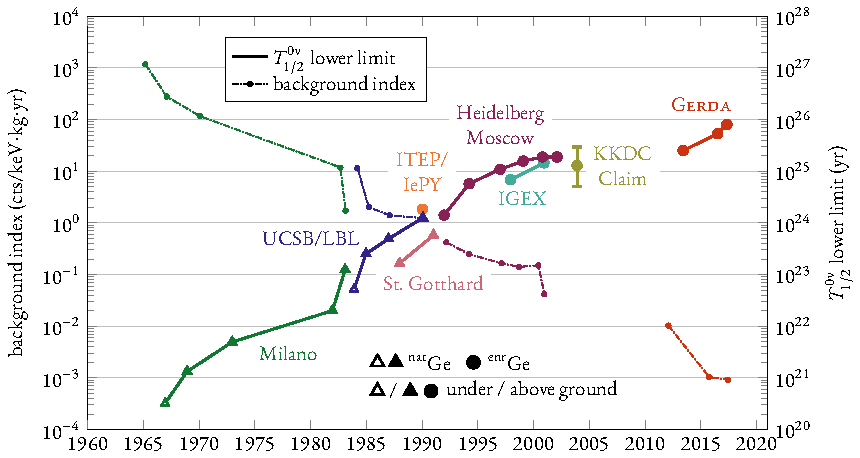
\includegraphics[width=\textwidth]{plots/history/0nbb-ge76-history.pdf}
  \end{center}
\end{frame}
\begin{frame}[plain]{\alert{GER}manium \alert{D}etector \alert{A}rray}
  \begin{columns}[c]
    \column{0.3\textwidth}%
      \begin{simpleblock}
        \begin{center}
          Enriched, high-purity \gesix\ detectors \\ \alert{source $=$ detector}
        \end{center}
      \end{simpleblock}
      \begin{itemize}
        \item Installed at LNGS (3500 m.w.e.), in activity since 2009
          \arrow\ \alert{\phaseone}
        \item Hardware upgrade 2015 \arrow\ \alert{\phasetwo}
        \item Decommissioned in 2020 \arrow\ \alert{LEGEND-200}
      \end{itemize}
    \column{0.7\textwidth}%
      \begin{center}
        \begin{tikzpicture}[fill=bg]
          \node at (0.1,0) {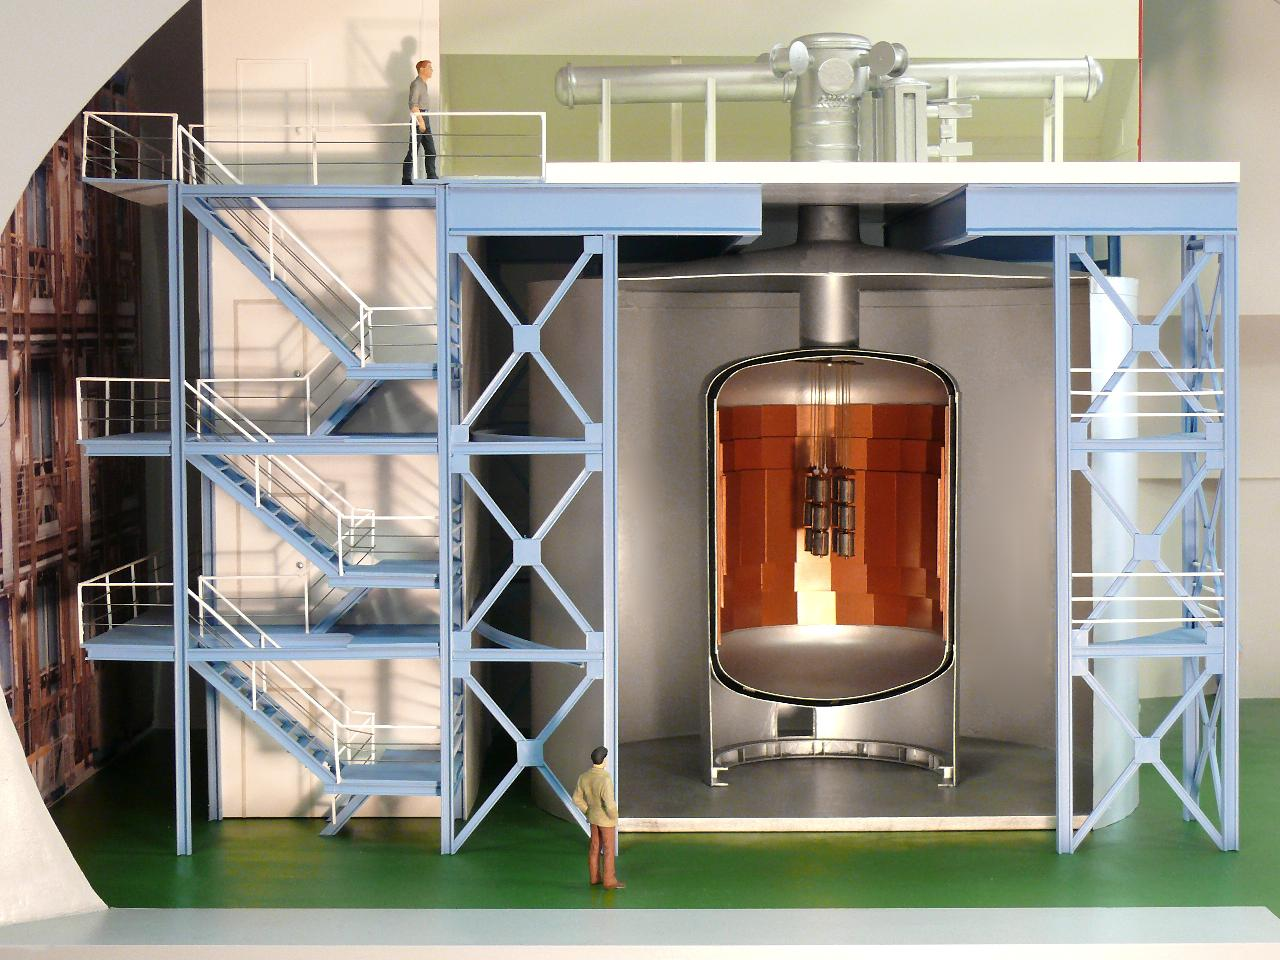
\includegraphics[height=7cm]{setup/gerda-artist.jpg}};
          \node(e) at (3.5,3.3) [rectangle,draw,fill] {\textsc{scintillators}};
          \draw[thick,red,->] (e.south) .. controls +(0,-1) and +(0,1) .. (2.5,2.3);
          \node(b) at (3.2,1.6) [rectangle,draw,fill] {\gesix\ \textsc{detectors}};
          \draw[thick,red,->] (b.south) .. controls +(0,0) and +(1,0) .. (1.7,-0.4);
          \node(c) at (-1.5,1.6) [rectangle,draw,fill] {H$_2$O};
          \draw[thick,red,->] (c.south) .. controls +(0,0) and +(-1,0) .. (0.2,-1);
          \node(d) at (0,3) [rectangle,draw,fill] {LAr};
          \draw[thick,red,->] (d.south) .. controls +(0,0) and +(-1,0) .. (1,-0.7);
          \node at (3,-3) [rectangle,draw=mLightBrown, fill=white] {Hosted at LNGS};
        \end{tikzpicture}
      \end{center}
  \end{columns}
\end{frame}
\begin{frame}[plain]{\alert{GER}manium \alert{D}etector \alert{A}rray at LNGS}
  \begin{center}
    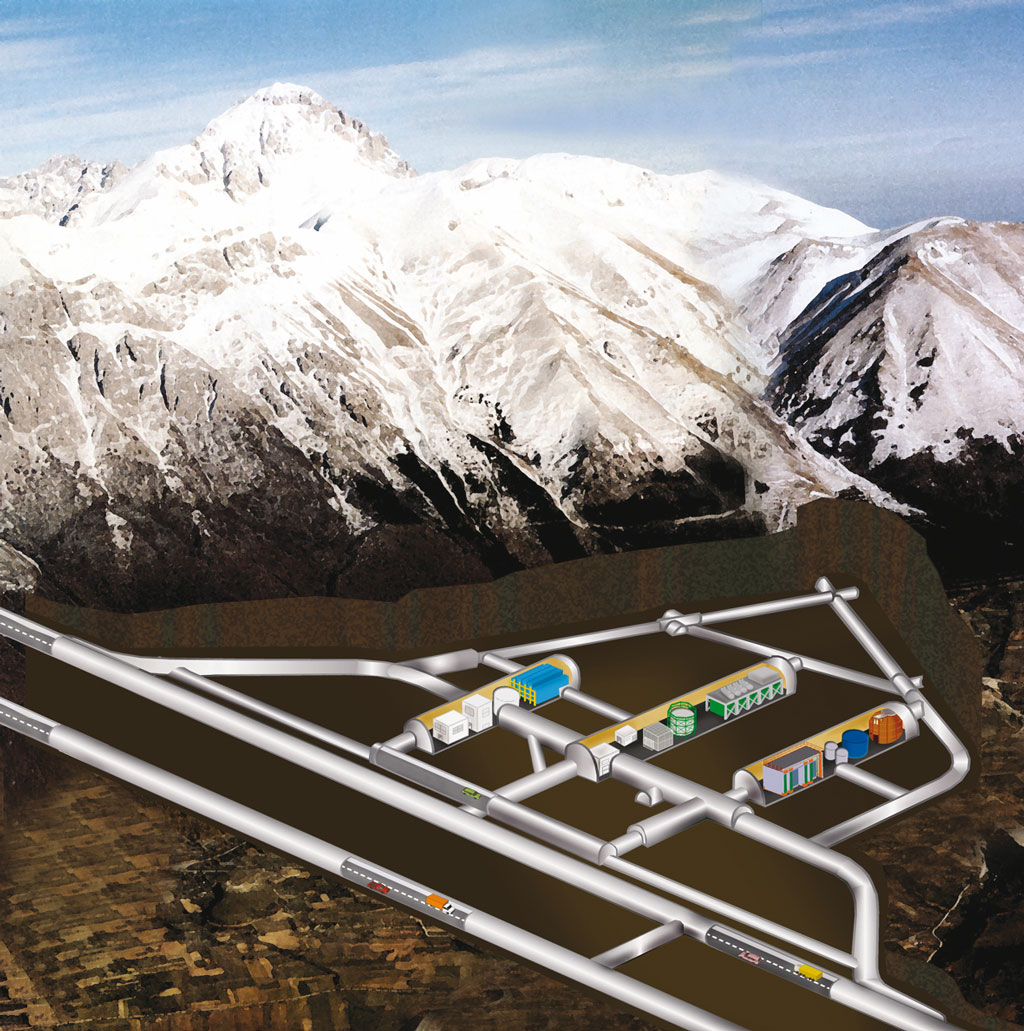
\includegraphics[height=0.95\textheight]{setup/lngs-map.jpg}
    \hspace{0.2cm}
    \includegraphics[height=0.95\textheight]{setup/gerda-lngs.jpg}
  \end{center}
\end{frame}
\begin{frame}{Signal and background discrimination techniques}
  \begin{center}
    \includegraphics[width=\textwidth]{setup/gerda-events.png}
  \end{center}
  \begin{simpleblock}
    \begin{center}
      \alert{\onbb} detection \alert{efficiency} between \alert{45--65\%}
      depending on the detector type
    \end{center}
  \end{simpleblock}
\end{frame}
\begin{frame}{Final results}
  \begin{columns}
    \begin{column}{0.45\textwidth}
      \begin{simpleblock}
        \href{https://doi.org/10.1103/PhysRevLett.125.252502}{\emph{Phys.~Rev.~Lett.}~125, 252502 (2020)}
      \end{simpleblock}
      \begin{itemize}
        \item New, advanced statistical analysis
        \item \alert{\measurement{5.2}{1.6}{1.3}~\powctsper{-4}} at \qbb
        \item No evidence for a signal with \alert{127.2~\kgyr} exposure
        \item \alert{$\thalfzeroM > \thalfzerolimit$~yr} (90\% C.L., frequentist)
        \item \mbb\ < 79--180~meV
      \end{itemize}
    \end{column}
    \begin{column}{0.55\textwidth}
      \begin{center}
        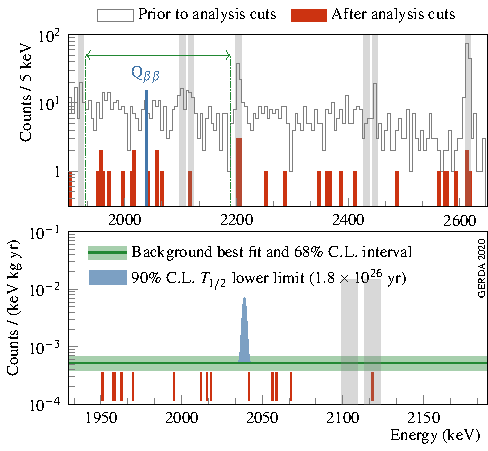
\includegraphics[width=\columnwidth]{plots/G2006_spectr_prl_2.pdf}
      \end{center}
    \end{column}
  \end{columns}
\end{frame}
\section{The background model before analysis cuts}
\begin{frame}{Motivations}
  \begin{simpleblock}\centering\itshape
    Can one claim the presence of a \textbf{signal} \\
    without understanding the \textbf{background}?
  \end{simpleblock}

  \vspace*{10pt}
  With the \textbf{background model} of \onbb\ experiments we want to\ldots
  \begin{itemize}
    \item Study the background composition at \alert{\qbb}
    \item Cross-check background \alert{intensity expectations}
    \item Characterize \alert{location} of background sources for future improvements
    \item Unveil the \alert{\nnbb} distribution and search for new physics signals
  \end{itemize}
\end{frame}
\begin{frame}[plain]{The \gerda\ data before cuts}
  \begin{center}
    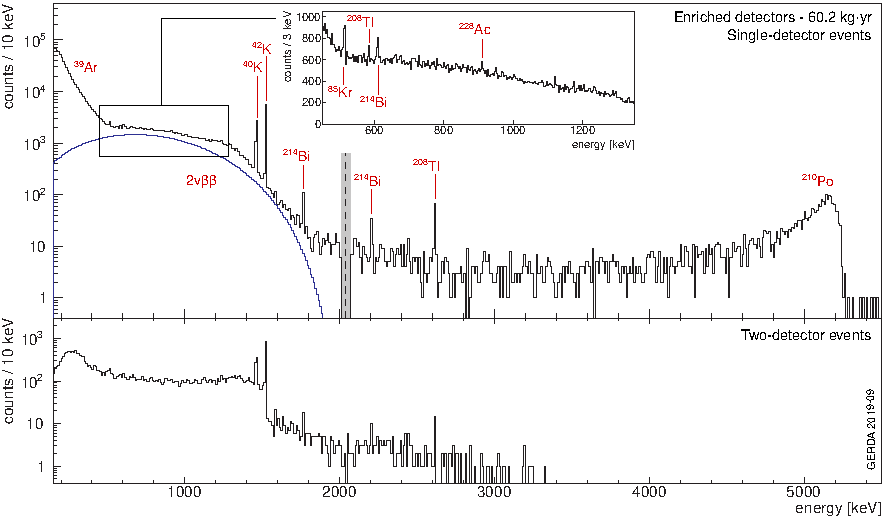
\includegraphics[height=0.95\textheight]{plots/bkg/raw/ph2/dataGe-desc.pdf}
  \end{center}
\end{frame}
\begin{frame}{Background expectations: Monte Carlo simulation}
  \begin{center}
    \begin{tikzpicture}[anchor=north west]
      \node at (0,0) {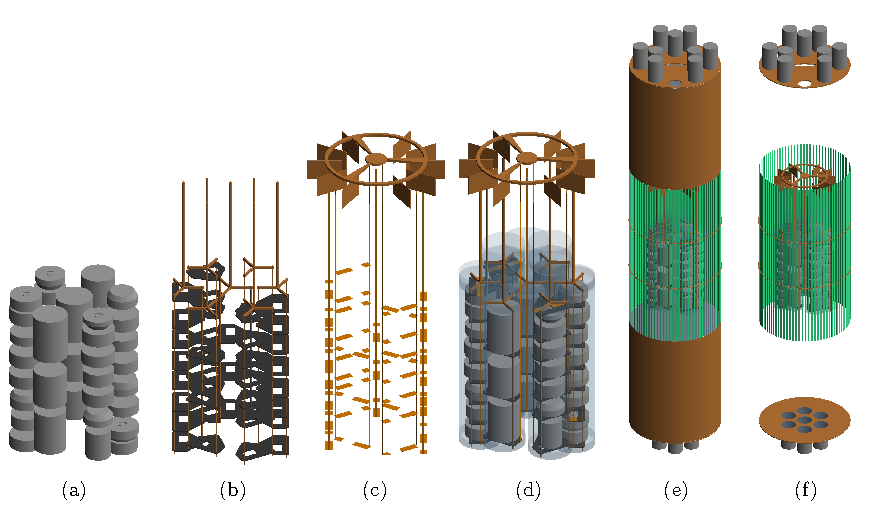
\includegraphics[trim=0 15 0 0, clip, width=0.95\textwidth]{setup/mage-volumes.pdf}};
      \node[align=center] at (1,0) {\mage: a \geant-based simulation framework \\ \href{https://doi.org/10.1109/TNS.2011.2144619}{\small\emph{IEEE Trans.~Nucl.~Sci.}~58 (2011) 1212-1220}};
    \end{tikzpicture}
  \end{center}
\end{frame}
\begin{frame}{Analysis strategy}
  \begin{center}
    \includegraphics[height=0.9\textheight]{plots/bkg/raw/combined-data.pdf}
  \end{center}
\end{frame}
\begin{frame}{Analysis strategy}
  \alert{Bayesian} analysis\footnote{With the Bayesian Analysis Toolkit (BAT):
  \url{https://bat.mpp.mpg.de}} with \emph{binned-likelihood} and \emph{priors}
  from material screening measurements
  \begin{description}
    \item[\a-model] \alert{high-energy events} (\a) on the \pplus\ contact
    \item[K-model] \alert{potassium full-energy peak} events divided by
      detector
    \item[global-model] final analysis on the \alert{full energy range},
      incorporates \a-model and K-model
  \end{description}

  \arrow\ Open-source fitting framework: \github{gipert/gerda-fitter}
\end{frame}
\begin{frame}{\a-model: coaxial detectors}
  \begin{simpleblock}
    \centering
    Combination of \pplus\ thicknesses well describes the data
  \end{simpleblock}
  \begin{center}
    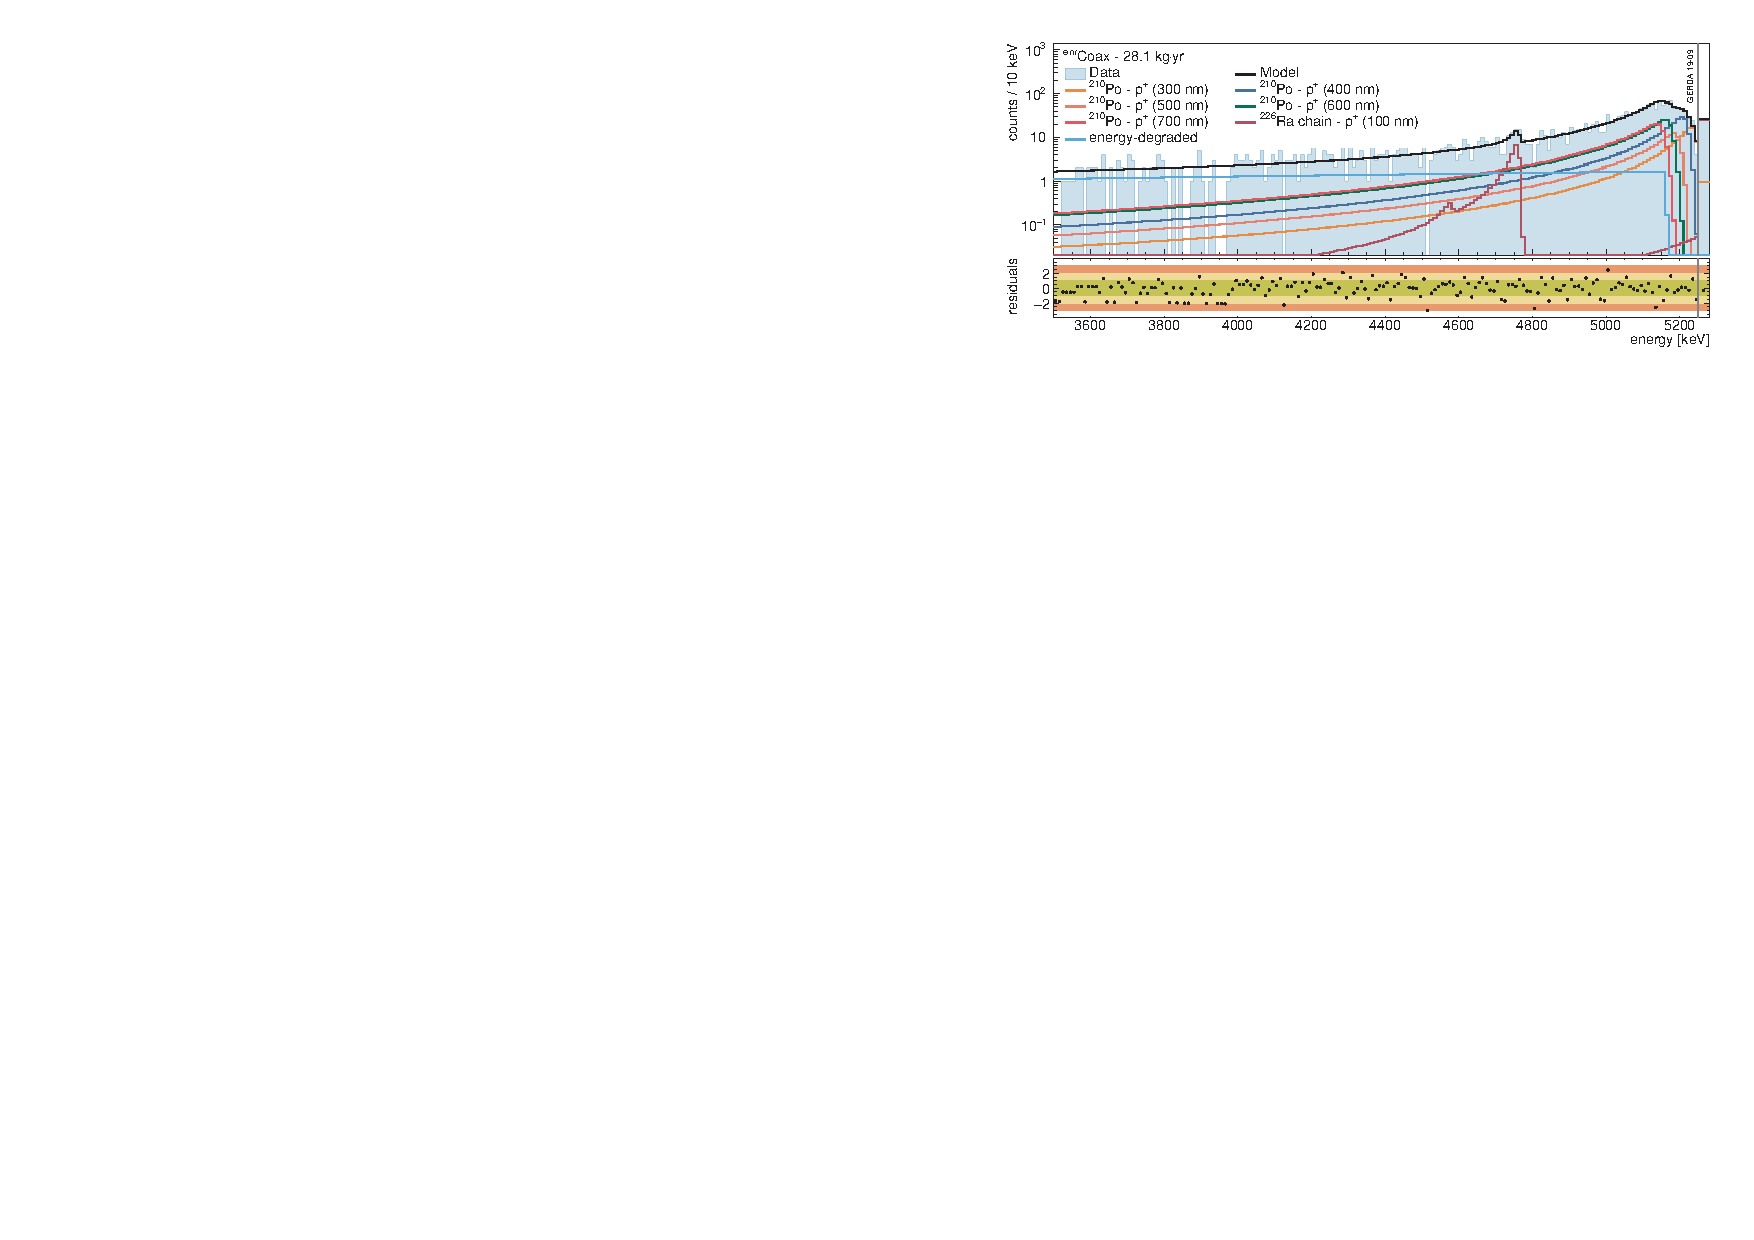
\includegraphics[width=0.9\textwidth]{plots/bkg/raw/ph2/results/amodel/amodel-enrCoax.pdf}
  \end{center}
\end{frame}
\begin{frame}{K-model: single-detector events}
  \begin{center}
    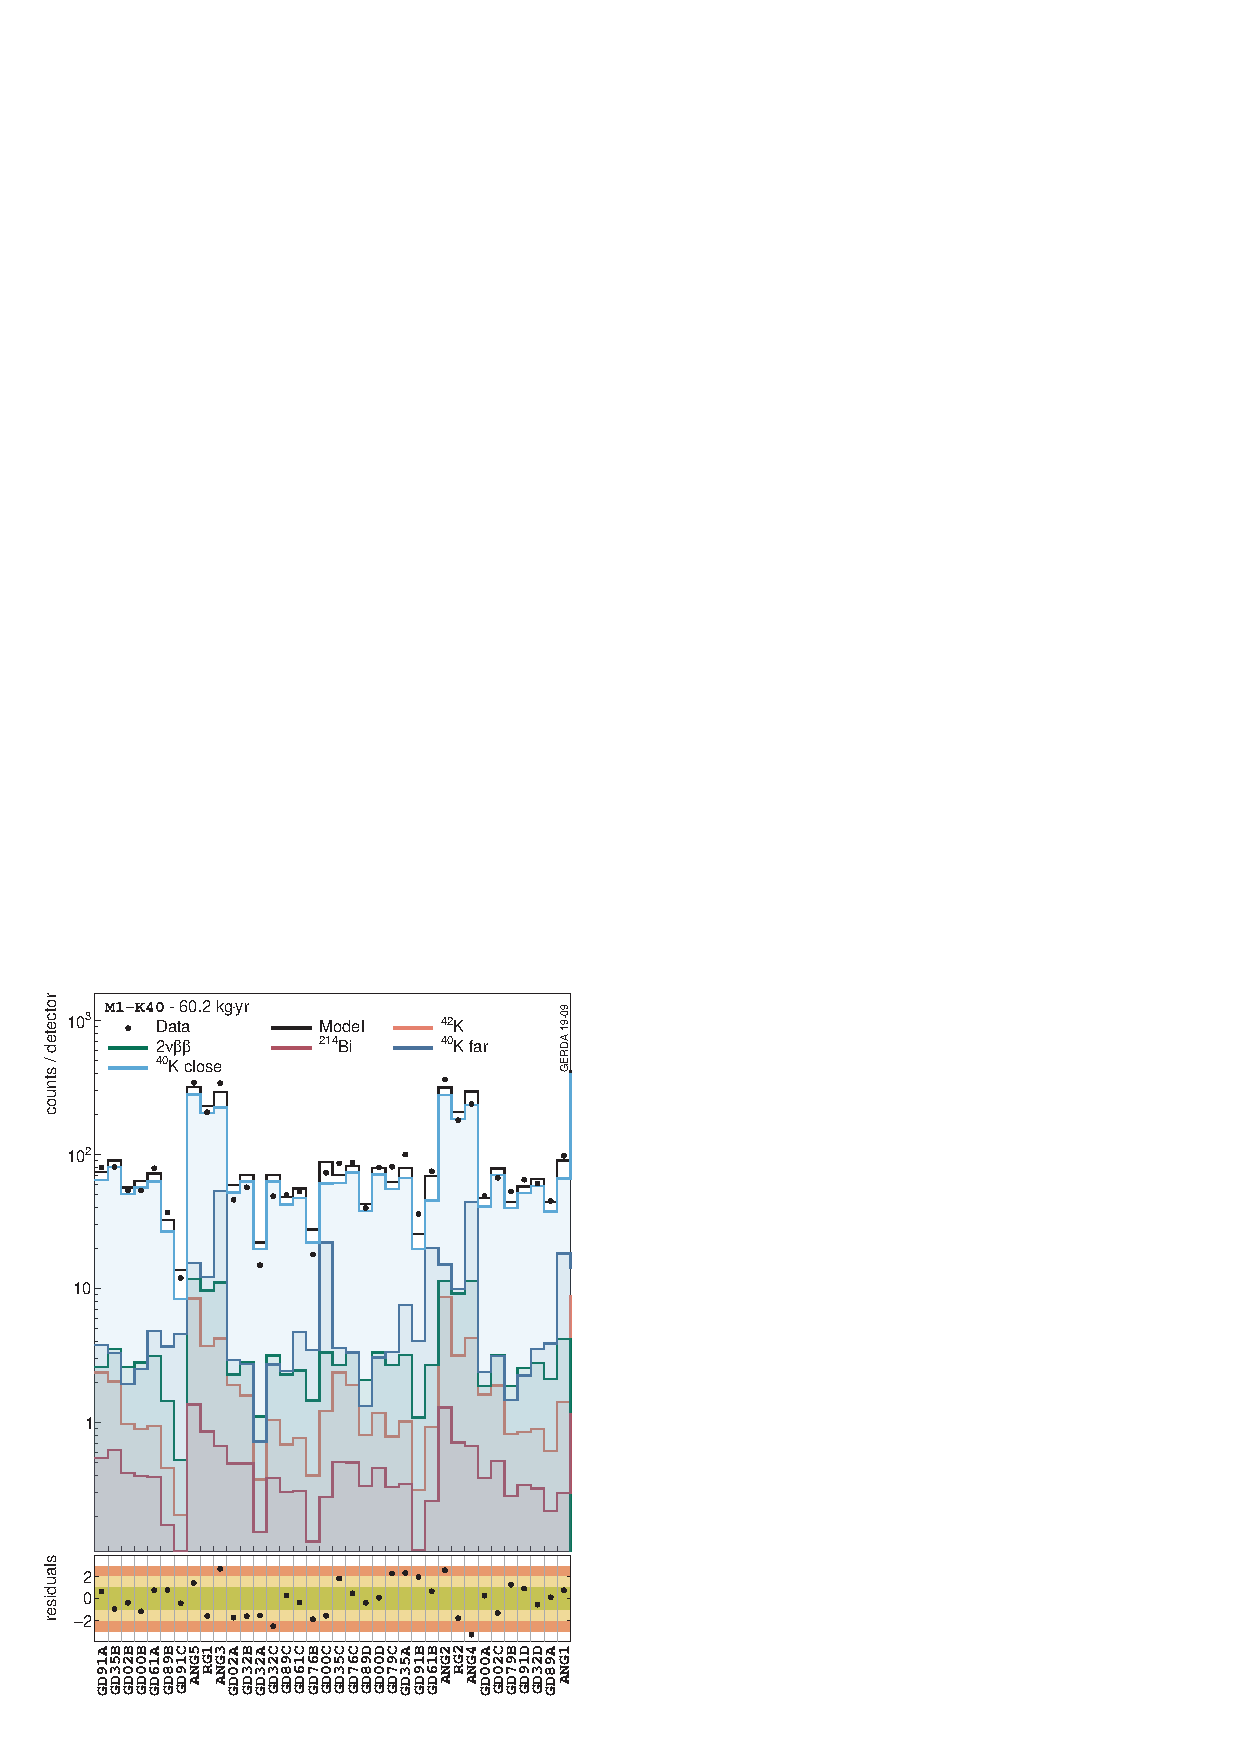
\includegraphics[height=0.85\textheight]{plots/bkg/raw/ph2/results/kmodel/kmodel-1d-ds0.pdf}
    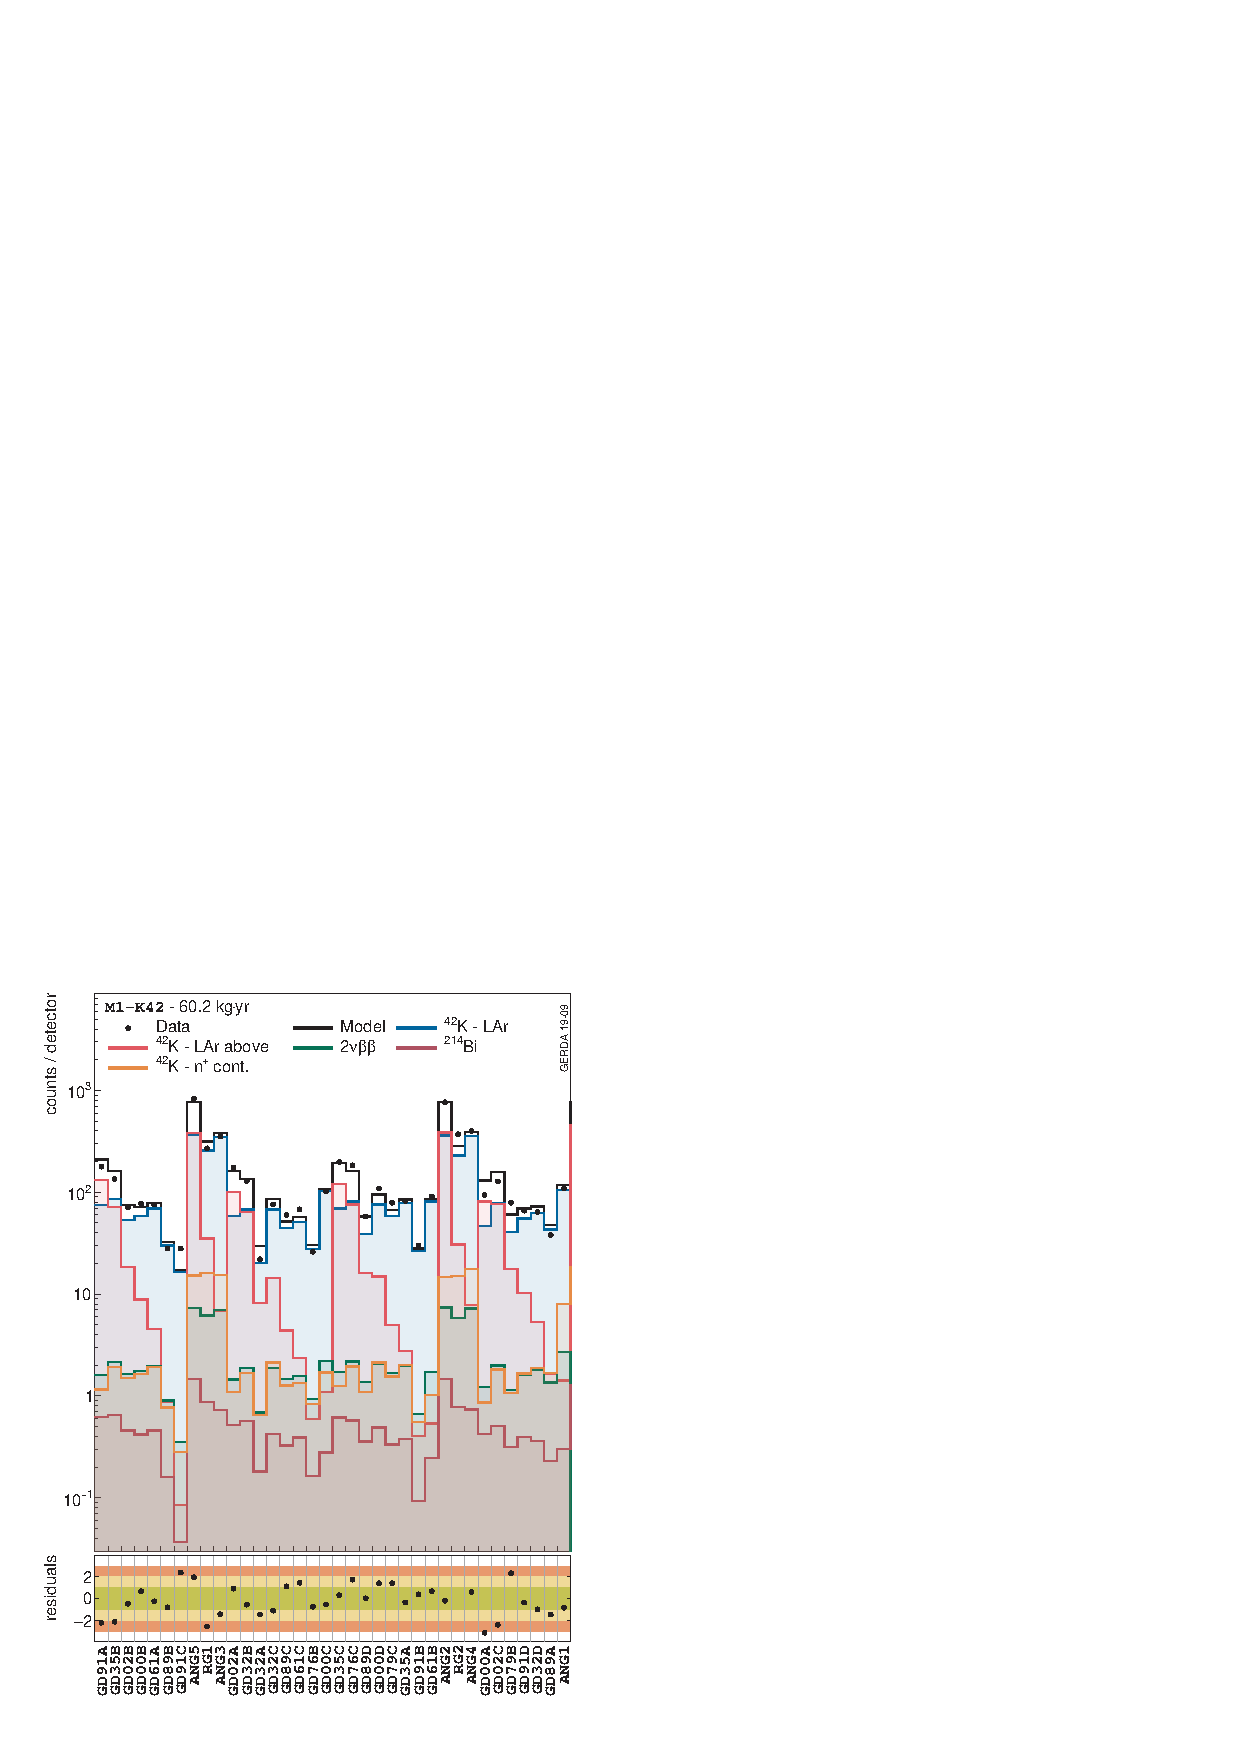
\includegraphics[height=0.85\textheight]{plots/bkg/raw/ph2/results/kmodel/kmodel-1d-ds1.pdf}
  \end{center}
\end{frame}
\begin{frame}[plain]{global-model: full \phasetwo\ dataset (\gexpobkg)}
  \begin{center}
    \includegraphics[height=0.9\textheight]{plots/bkg/raw/combined-results.pdf}
  \end{center}
\end{frame}
\begin{frame}{Things that we have learned}
  \begin{columns}
    \begin{column}{0.64\textwidth}
      \vspace*{-0.7cm} \\
      \begin{simpleblock}\centering
        \href{https://doi.org/10.1007/JHEP03(2020)139}{\emph{J.~High~Energ.~Phys.}~03 (2020) 139}
      \end{simpleblock}
      \begin{itemize}
        \item Excellent goodness-of-fit, \alert{we understand our background}
        \item Screening measurements reproduced, except for \kvn
        \item Inhomogeneous \kvz\ distribution
        \item Indication of a biased \bege\ active volume size
      \end{itemize}
    \end{column}
    \begin{column}{0.36\textwidth}
      \vspace*{1.6cm} \\
      \fbox{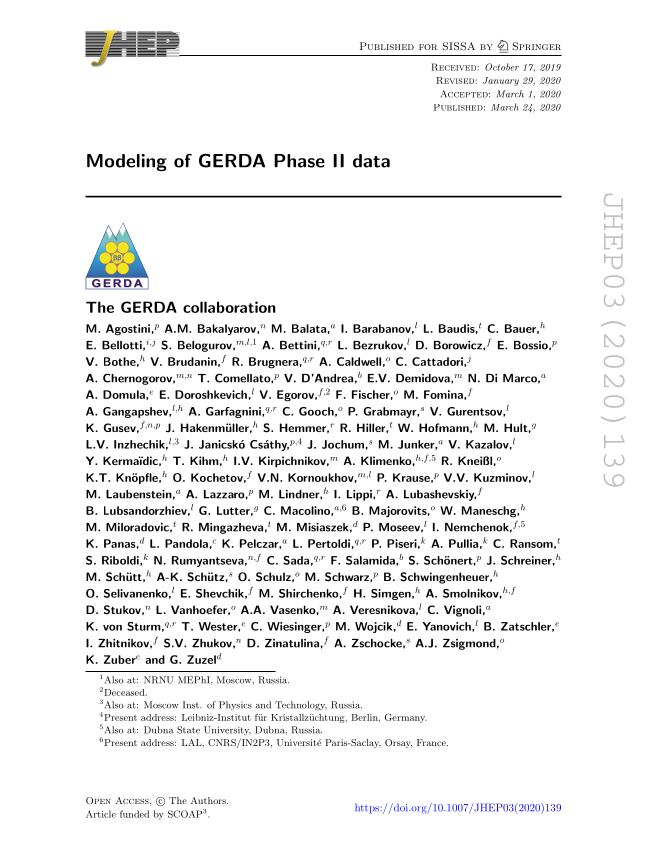
\includegraphics[width=4.5cm,clip,trim=0 0 0 0]{jhep-paper.png}}
    \end{column}
  \end{columns}
\end{frame}
\section{The background model after the LAr veto cut}
\begin{frame}{The scintillation of liquid argon (LAr)}
  Liquid argon as a \emph{cooling medium}, \emph{passive shield} against
  backgrounds (\phaseone) and \alert{active shield} (\phasetwo).
  \begin{center}
    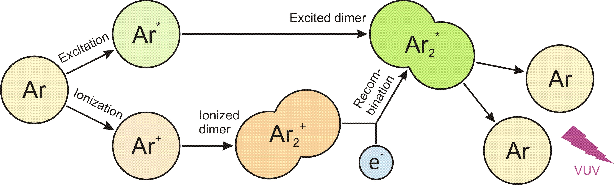
\includegraphics[width=0.8\textwidth]{lar-scint-mechanism.pdf}
  \end{center}
  \arrow\ light is produced at the passage of ionizing radiation,
  \emph{detector medium}
\end{frame}
\begin{frame}{Collecting the LAr scintillation light}
  \tikzstyle{every picture}+=[remember picture]
  \tikzstyle{na} = [baseline=-.5ex]
  \begin{columns}%
    \column{0.55\textwidth}%
      \begin{itemize}
        \item<1-> 16 \alert{PMTs} \tikz[na] \node[coordinate] (n1) {};
        \item<2-> light-guiding \alert{fibers} + SiPM readout \tikz[na]
          \node[coordinate] (n2) {};
        \item<3-> nylon \alert{mini-shrouds} for each string \tikz[na]
          \node[coordinate] (n3) {}; \\
          \arrow\ mechanical barrier against \kvz\ ions
      \end{itemize}
    \column{0.45\textwidth}%
        \begin{tikzpicture}
          \node (t1) at (0,2.8)  {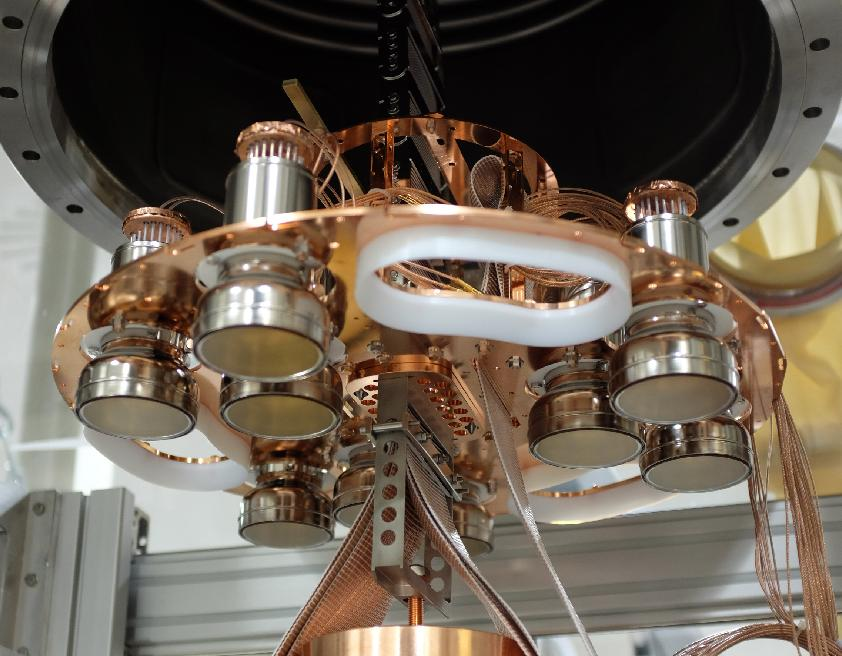
\includegraphics[width=2cm]{setup/larveto-top-pic.jpg}};
          \node (t2) at (0.0,0)  {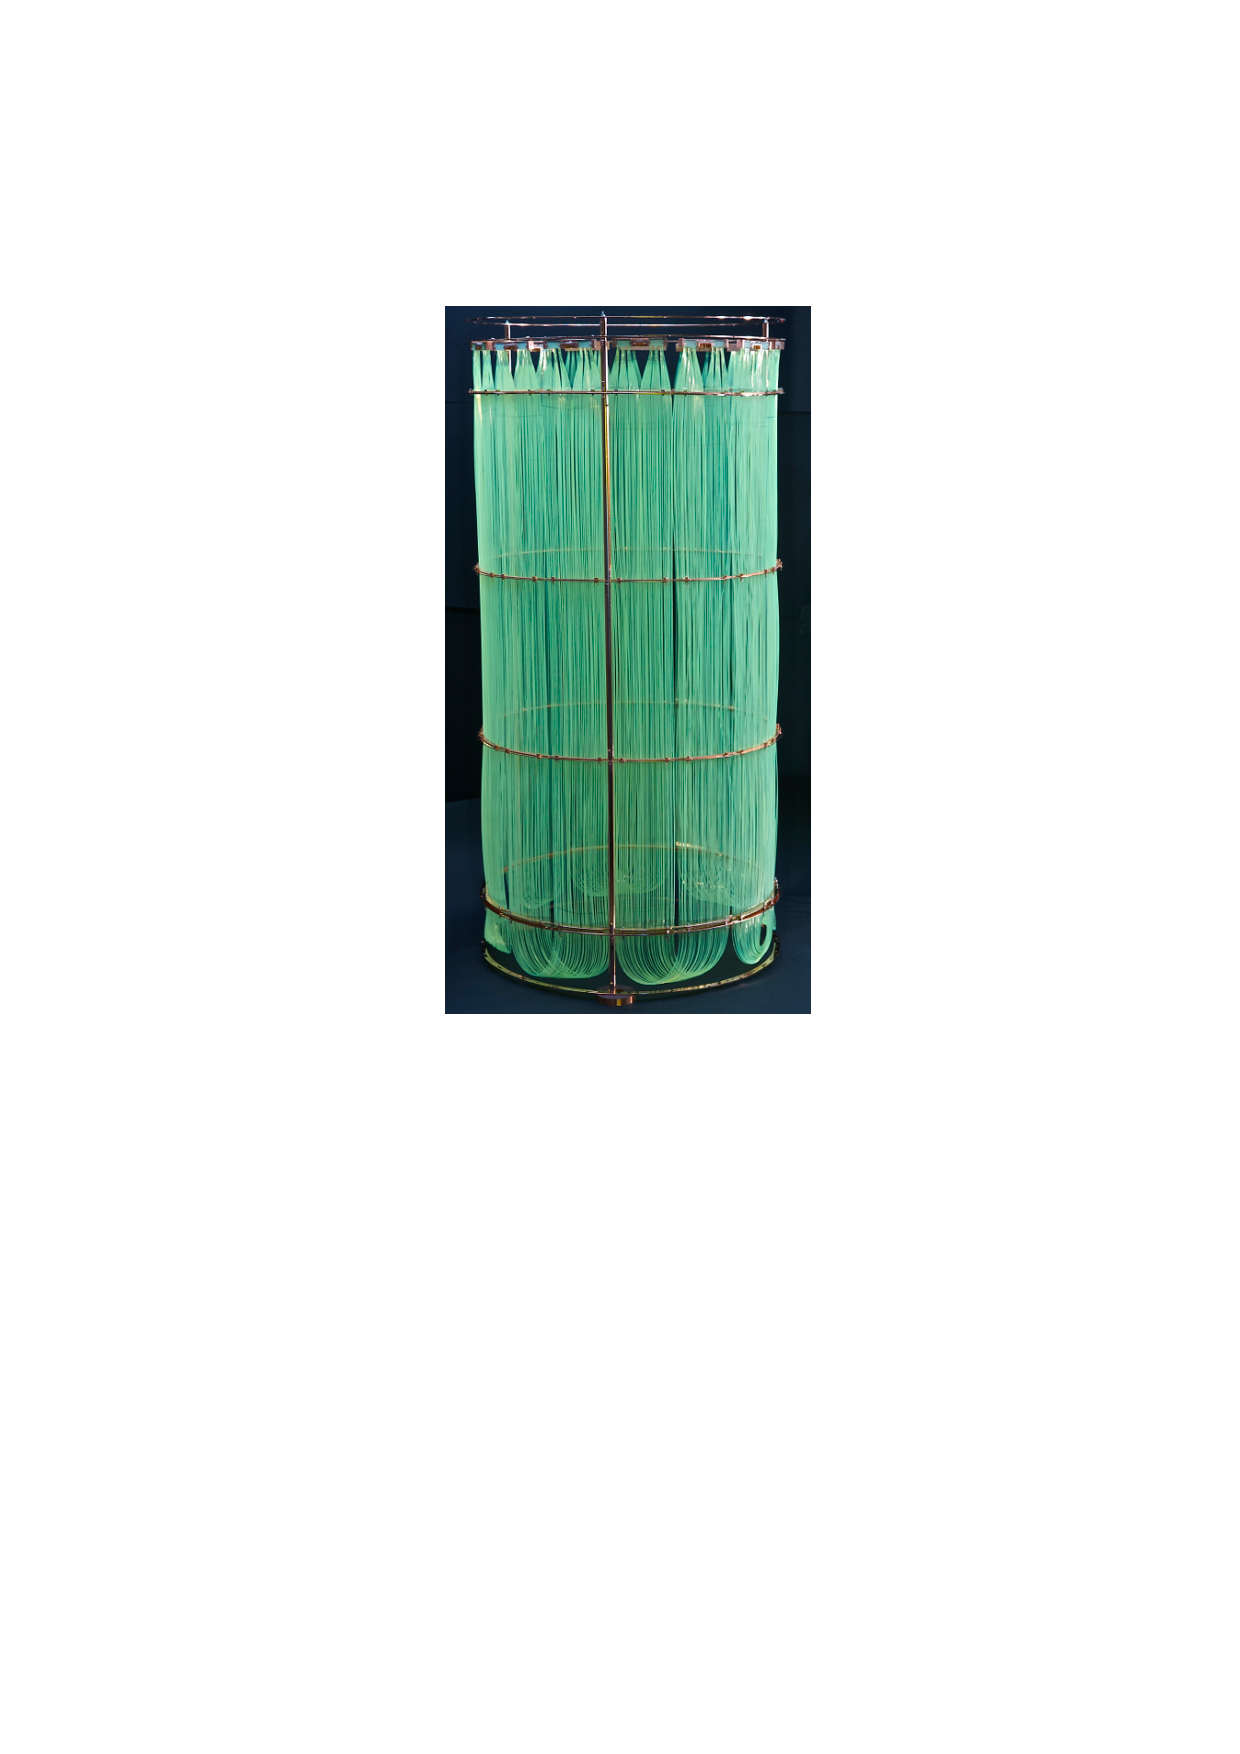
\includegraphics[width=2cm]{setup/fibers-pic.pdf}};
          \node (t3) at (0,-2.6) {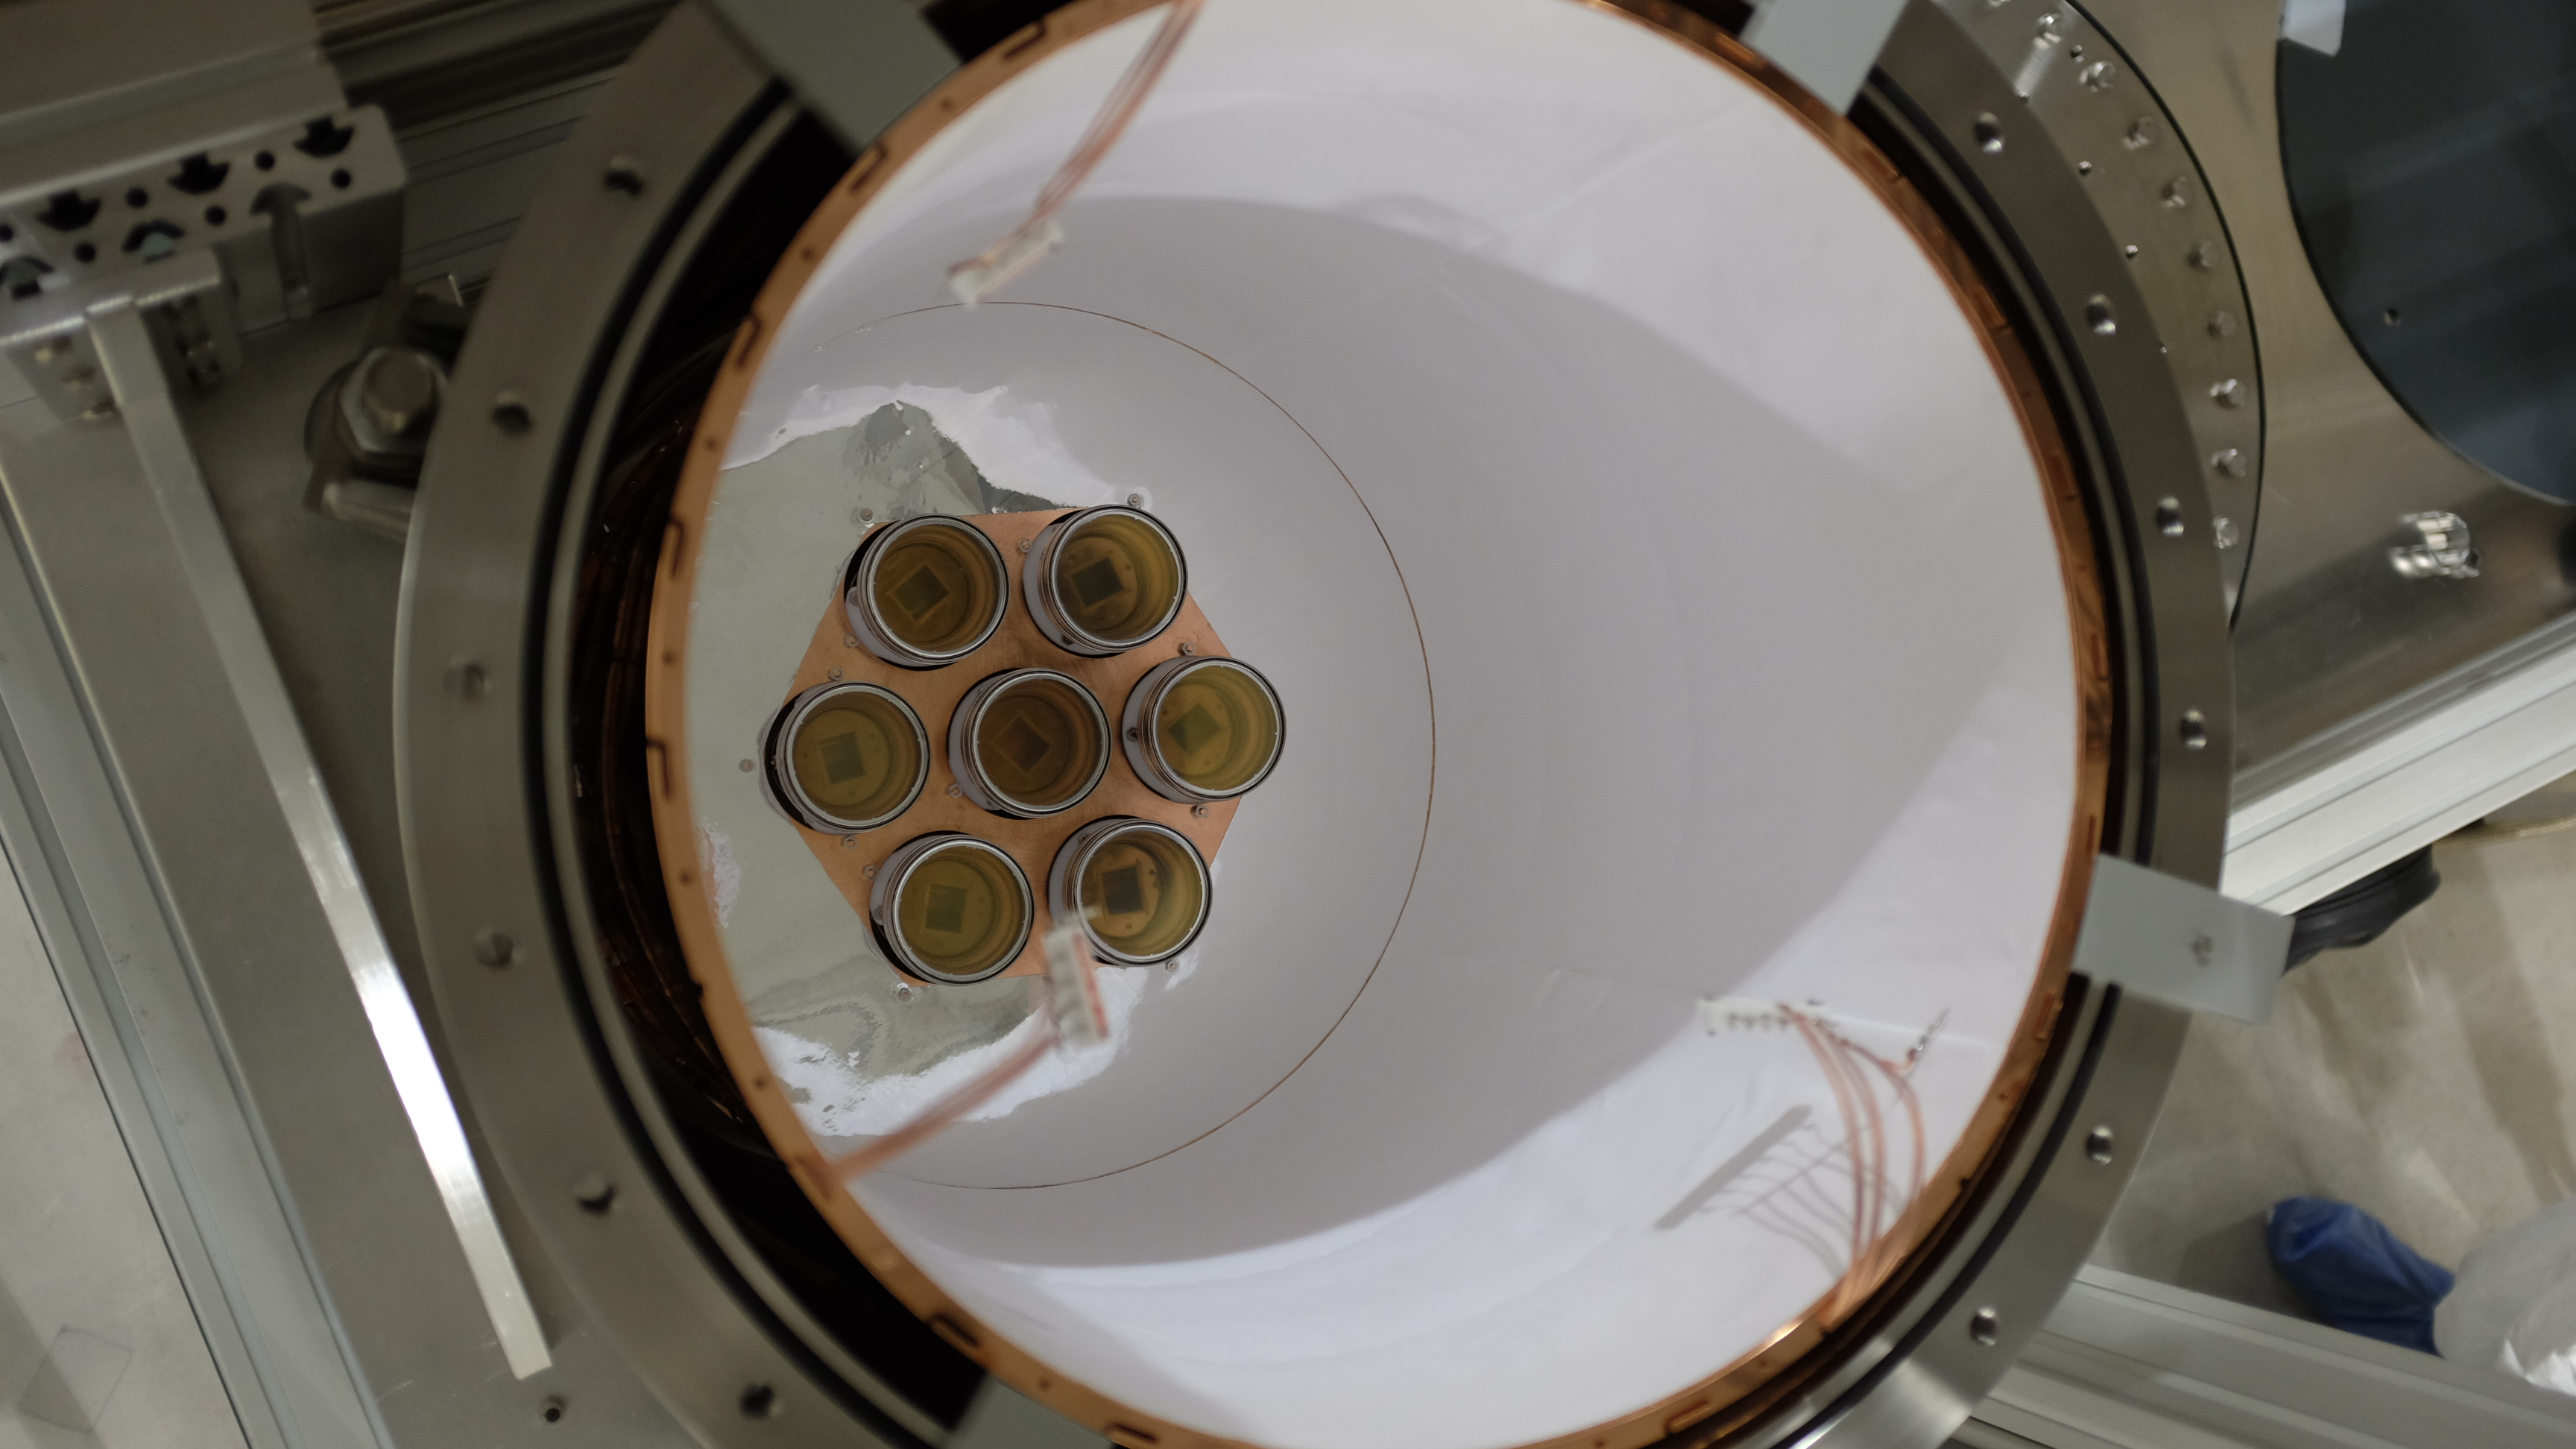
\includegraphics[width=2cm]{setup/larveto-bottom-pic.jpg}};
          \node (t4) at (2.5,0)  {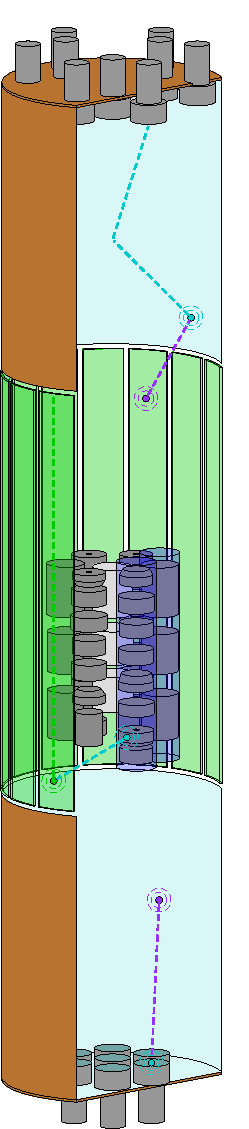
\includegraphics[height=0.95\textheight]{setup/lar-veto-tikz.pdf}};
          \node (t5) at (-2.1,0) {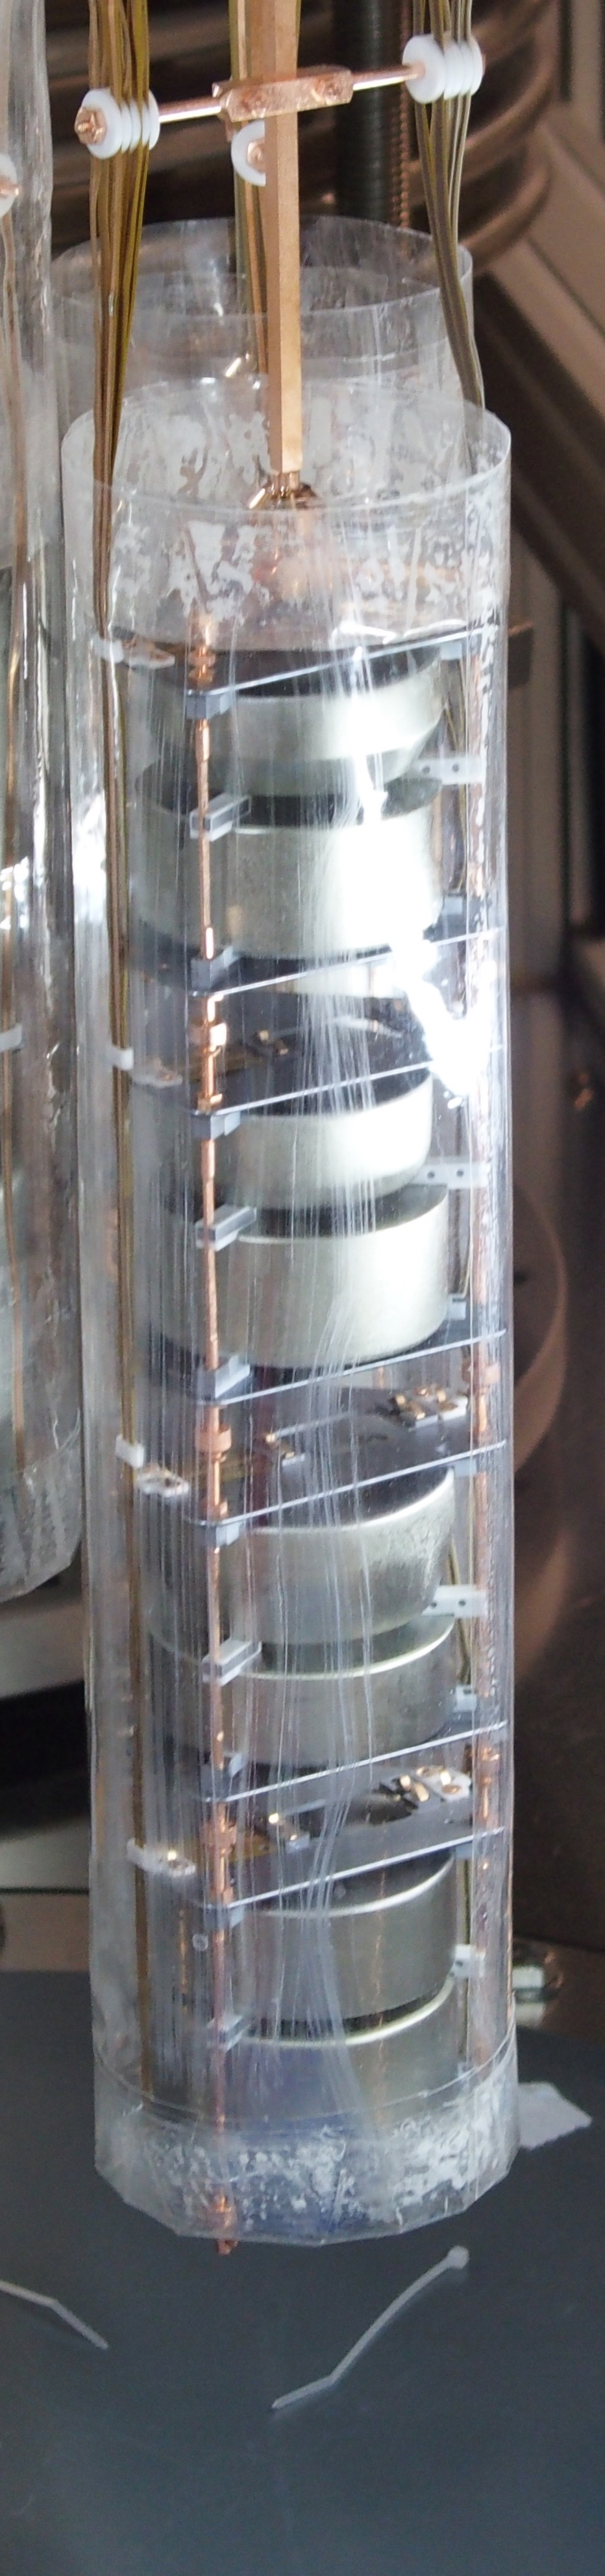
\includegraphics[width=1.3cm]{setup/ms-pic.jpg}};
        \end{tikzpicture}
  \end{columns}
  \begin{tikzpicture}[overlay,very thick,color=mLightBrown]
    \path[->]<1> (n1) edge [out=0, in=160] (t1);
    \path[->]<1> (n1) edge [out=0, in=200] (t3);
    \path[->]<2> (n2) edge [out=0] (t2);
    \path[->]<3> (n3) edge [out=0] (t5);
  \end{tikzpicture}
\end{frame}
\begin{frame}{The data after the LAr veto cut}
  \begin{columns}
    \begin{column}{0.7\textwidth}\setlength{\parskip}{10pt}%
      \begin{exampleblock}{LAr veto cut definition}
        Ge events with coincident light detection in LAr are cut (No light is
        expected from \b\b-decay events)
      \end{exampleblock}

      Removes a lot of background in the \nnbb\ energy region \\
      $\Rightarrow$ \alert{higher sensitivity to (new) physics searches}
      (exotic \nnbb\ decays, \b\b-decays to excited states\ldots)
    \end{column}
    \begin{column}{0.3\textwidth}\centering
      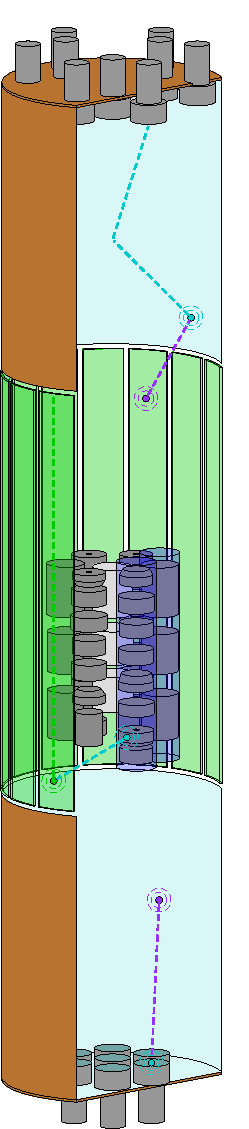
\includegraphics[width=3cm,clip,trim=0 220 0 0]{setup/lar-veto-tikz.pdf}
    \end{column}
  \end{columns}
\end{frame}
\begin{frame}{The data after the LAr veto cut}
  \centering
  \includegraphics[height=0.9\textheight]{plots/bkg/lar/combined-data.pdf}
\end{frame}
\begin{frame}{The data after the LAr veto cut}
  \begin{columns}
    \begin{column}{0.7\textwidth}\setlength{\parskip}{10pt}%
      \centering
      \includegraphics[width=\columnwidth]{plots/bkg/lar/combined-data-zoom.pdf}
    \end{column}
    \begin{column}{0.3\textwidth}\centering
      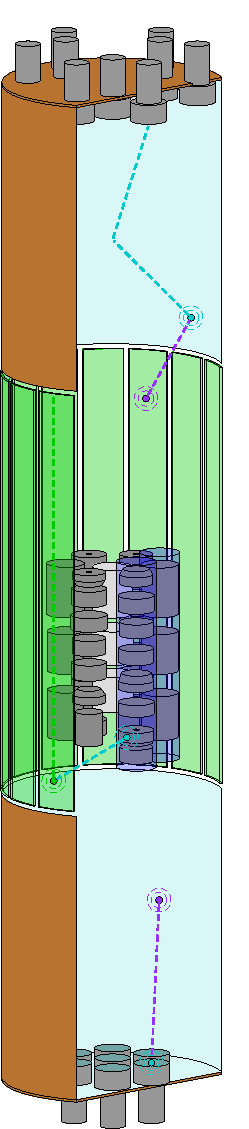
\includegraphics[width=3cm,clip,trim=0 220 0 0]{setup/lar-veto-tikz.pdf}
    \end{column}
  \end{columns}
\end{frame}
\begin{frame}{Simulating the LAr scintillation}
  \begin{columns}
    \begin{column}{0.6\textwidth}\setlength{\parskip}{10pt}%
    Once optical specifications are implemented, photon tracking can be enabled
    in \geant. Problem:
    \begin{center}
      \alert{it's SLOW} {\small(on CPUs)}
    \end{center}
    too many photons to track! Typical simulation rate of scintillation photons
    in the \gerda\ setup is \alert{100 ph/s}.

    \emph{Can we be smart and pre-compute the information we really need?}
    \end{column}
    \begin{column}{0.4\textwidth}
      \begin{center}
        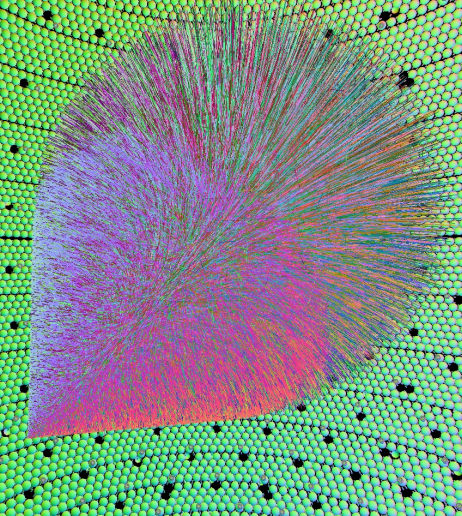
\includegraphics[width=\columnwidth]{opticks-shower.png}
      \end{center}
    \end{column}
  \end{columns}
\end{frame}
\begin{frame}{Simulating the LAr veto flag: probability map approach}
  The LAr probability map: Track optical photons once and for all:
  \begin{itemize}
    \item Directly simulate \alert{128~nm} scintillation photons in LAr
    \item Partition the LAr volume in \alert{voxels} ($\sim3^3$ mm$^3$)
    \item Calculate LAr veto \alert{detection probability} for a photon in a voxel
  \end{itemize}
  Still\ldots
  \begin{itemize}
    \item Computationally intensive, probabilities are generally very low
    \item Several thousands of CPU hours are needed to produce a map
  \end{itemize}
\end{frame}
\begin{frame}{Simulating the LAr veto flag: probability map approach}
  \begin{center}
    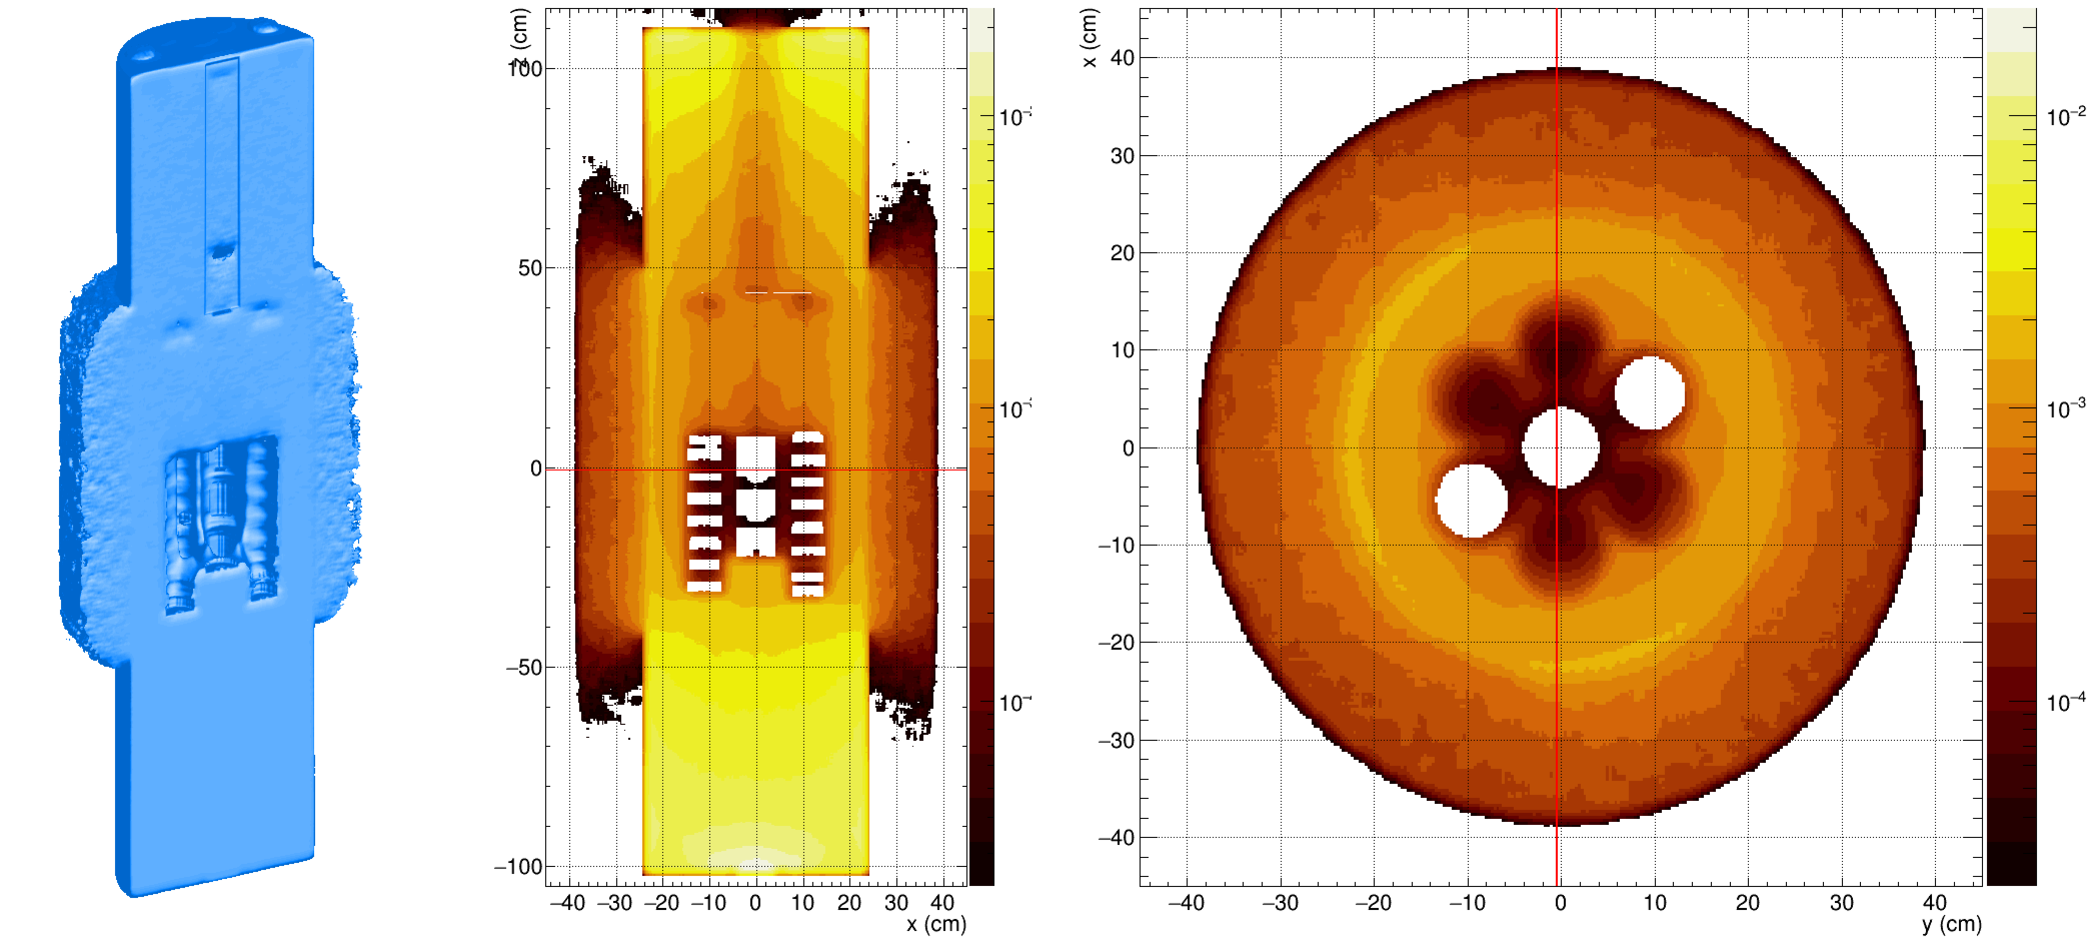
\includegraphics[width=\textwidth]{plots/bkg/lar/ph2/larmodel/larmap-tac.png}
  \end{center}
\end{frame}
\begin{frame}{Simulating the LAr veto flag: probability map approach}
  \begin{columns}
    \begin{column}{0.45\textwidth}
      From the probability map to the LAr veto flag:
      \begin{itemize}
        \item A Monte Carlo event deposits energy in LAr
        \item \# of photons determined with nominal light yield ($\sim$28
          ph/keV)
        \item Use the map to determine how many get detected
          (statistical)
        \item If detected $\geq 1 \Rightarrow$ vetoed
      \end{itemize}
    \end{column}
    \begin{column}{0.55\textwidth}
      \centering
      \vspace*{0.5cm} \\
      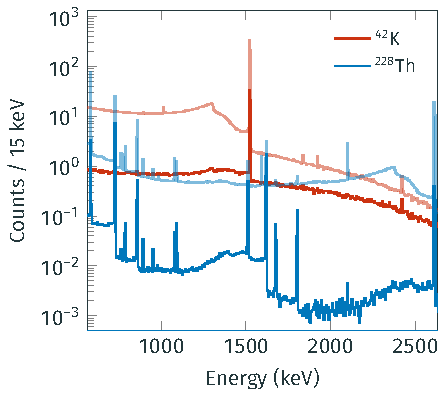
\includegraphics{plots/bkg/lar/pdfs-example.pdf}
    \end{column}
  \end{columns}
\end{frame}
\begin{frame}{Tuning the probability map with calibration data}
  \begin{simpleblock}
    The Monte Carlo parameters which are completely missing are the SiPMs and
    PMTs \alert{channel efficiencies} \arrow\ need to be extracted from real
    data\footnote{Note: we are not able to say something precise about the
    other MC parameters (LAr attenuation length, fiber coverage etc.), and it's
    definitely easier to constrain them with independent measurements.}
  \end{simpleblock}

  \vspace*{0.5cm}
  \begin{columns}
    \begin{column}{0.7\textwidth}\setlength{\parskip}{10pt}%
      \m{run68} and \m{run76} are special calibration runs with LAr veto ON and
      weak $\mathcal{O}(1)$~kBq radioactive sources
      \begin{description}
        \item[\m{run68}] \Th\ source, in Jul 2016
        \item[\m{run76}] \Ra\ source, in Feb 2017
      \end{description}

      \alert{\arrow\ Natural candidate LAr veto model tuning datasets}
    \end{column}
    \begin{column}{0.25\textwidth}
      \hspace{-0.5cm}\includegraphics[width=\columnwidth]{gedet/phII-array-calib.png}
    \end{column}
  \end{columns}
\end{frame}
\begin{frame}[plain]{global-model --- partial \phasetwo\ dataset (\gexpophasetwobkg)}
  \begin{center}
    \includegraphics[height=0.9\textheight]{plots/bkg/lar/combined-results.pdf}
  \end{center}
\end{frame}
\section{Precision fit of \texorpdfstring{\nnbb}{2nubb} events: standard and new physics}
\begin{frame}{Motivations}
  \begin{exampleblock}{Motivations\footnote{Legacy of analogous analysis of \gerda\ \phaseone\
    data, see \href{https://doi.org/10.1140/epjc/s10052-015-3627-y}{\emph{Eur.~Phys.~J.~C} 75, 416 (2015)}}}
    \begin{itemize}
      \item \textbf{High-statistics \nnbb\ sample:} $\sim$50 000 events in \bege\ detectors\footnote{Above the \Arl\ Q-value}
      \item \textbf{Low background level:} signal-to-background ratio of $\sim$20 ($\sim$2 before the cut)
    \end{itemize}
  \end{exampleblock}

  \begin{alertblock}{Science goal}
    \begin{itemize}
      \item Precision measurement of the Standard Model \textbf{\nnbb\ half-life}, shape check
      \item Constraints on \textbf{new-physics} models (Majorons, Lorentz violation\ldots)
    \end{itemize}
  \end{alertblock}
\end{frame}
\begin{frame}{Analysis strategy}
  \begin{columns}
    \hspace{-1cm}
    \begin{column}{0.6\textwidth}
      \begin{description}
        \item[Dataset] First \alert{32.7~\kgyr} from \phasetwo\ \alert{\bege\
          single-detector} event data
        \item[Likelihood] Usual binned-Poisson
          \[
            \mathcal{L}(S, \vec{B} | \vec{n}) =
            \prod_i^{N} \frac{{\nu_i(S, \vec{B})}^{n_i} e^{\nu_i(S, \vec{B})}}{n_i!}
          \]
        \item[Test statistic] Standard \alert{$t_S = -2\log\lambda(S)$} where
          $\lambda(S)$ is the \alert{profile likelihood ratio}. Sampled with MC
          methods
      \end{description}
    \end{column}
    \hspace{-2cm}
    \begin{column}{0.4\textwidth}
      \vspace*{1cm} \\
      \includegraphics{plots/bkg/lar/enrBEGe-data.pdf}
    \end{column}
  \end{columns}
\end{frame}
\begin{frame}{Inclusion of systematic uncertainties}
  \begin{columns}
    \begin{column}{0.55\textwidth}
      \begin{alertblock}{Hybrid Bayesian-frequentist approach}
        Sample toy data from systematically distorted models,
        according to ``prior'' distributions
        \[
          f(t_s) = \int f(t_s | S, \vec{B}, \nu) \cdot \pi(\vec{\nu}) \, d\vec{\nu}
        \]
      \end{alertblock}
      \begin{itemize}
        \item \textbf{Effect:} $f(t_S)$ smearing, weaker confidence intervals
        \item\github{gipert/gerda-factory}
      \end{itemize}
    \end{column}
    \begin{column}{0.45\textwidth}
      \centering
      \vspace*{0.5cm} \\
      \includegraphics[width=\columnwidth]{plots/2nbb-ana/bege-pdf-dist.pdf}
    \end{column}
  \end{columns}
\end{frame}
\begin{frame}{Example: LAr veto model uncertainties}
  \begin{columns}
    \begin{column}{0.85\textwidth}
      \begin{center}
        \includegraphics[width=\columnwidth]{plots/bkg/lar/ph2/larmodel/larmap-dist.pdf}
      \end{center}
      Simulations parameters have \emph{local} and \emph{global} effects
      \arrow\ systematic uncertainty \alert{distorts} the map
    \end{column}
    \begin{column}{0.15\textwidth}
      \begin{center}
        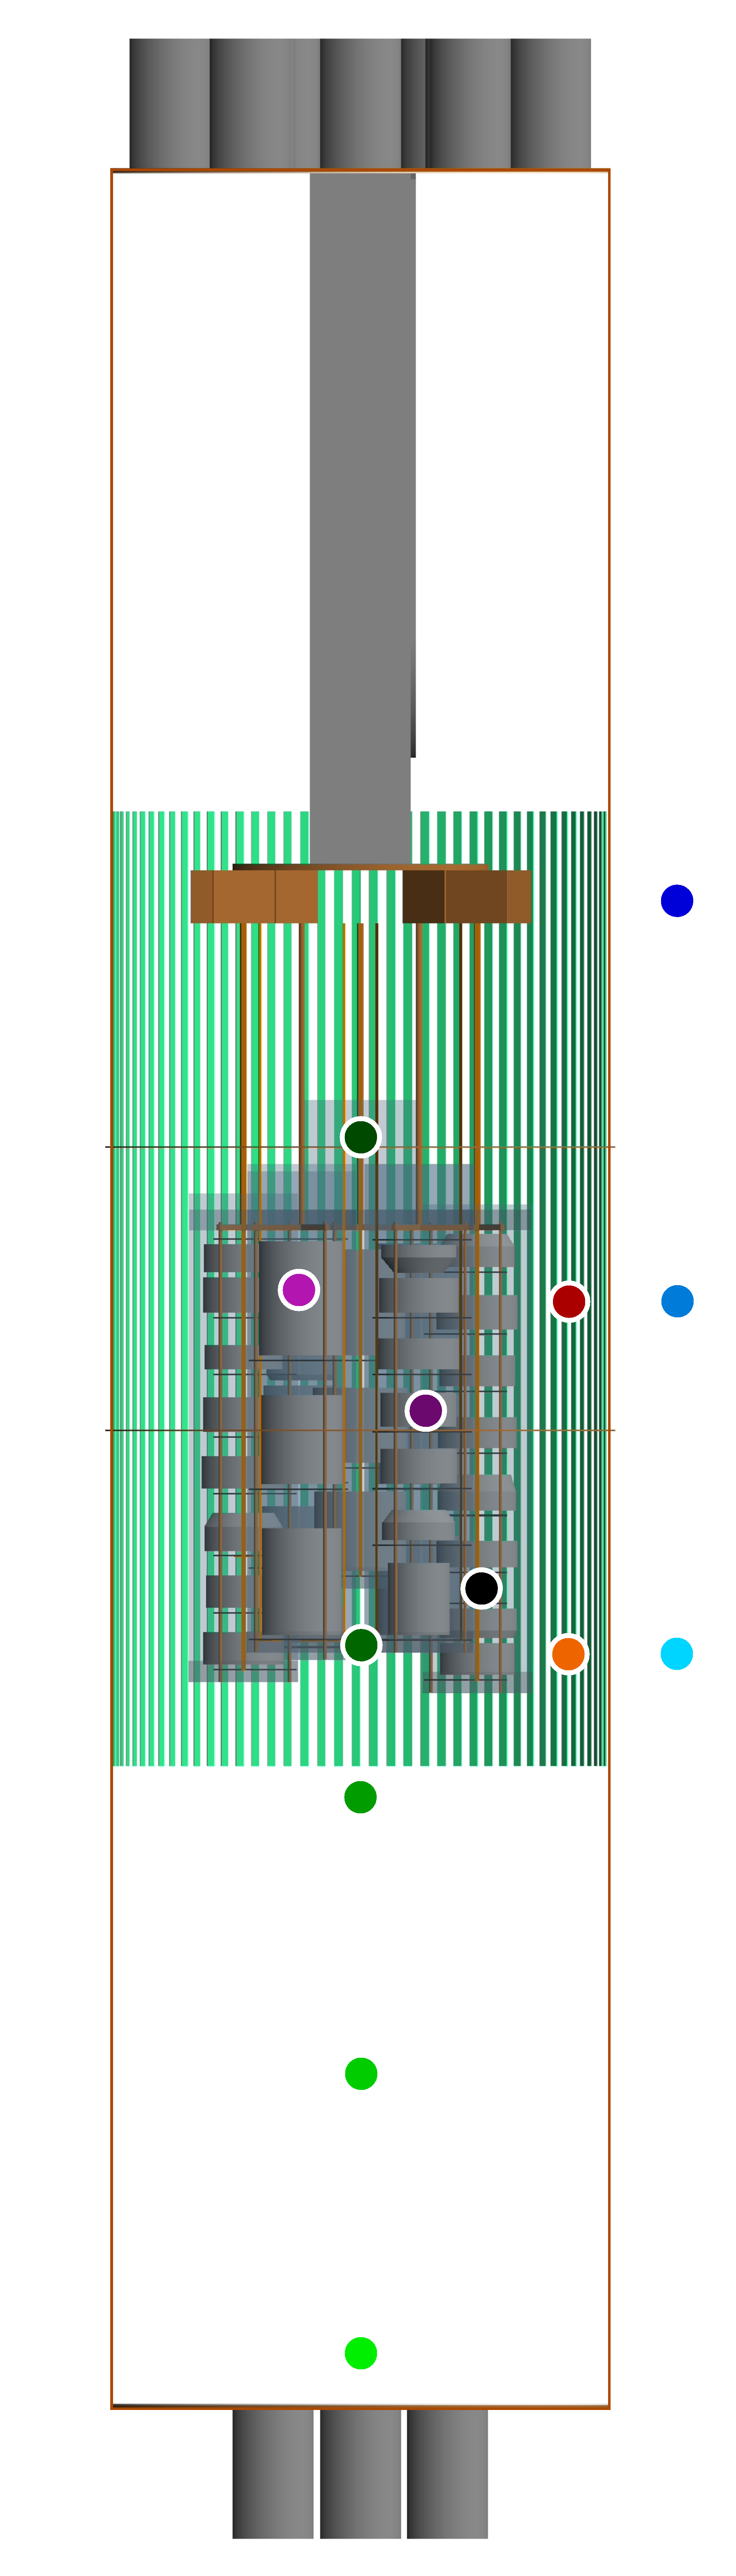
\includegraphics[height=0.9\textheight]{plots/bkg/lar/ph2/larmodel/lar-points-position.pdf}
      \end{center}
    \end{column}
  \end{columns}
\end{frame}
\begin{frame}{Example: LAr veto model uncertainties}
  The map generation is computationally expensive ($\mathcal{O}{(10^4)}$ CPU
  hours), we can produce only one from scratch \arrow\ what about
  \emph{artificial}, power-law\footnote{$p_k \rightarrow c \cdot p_k^a$ where
  $p$ is the detection probability and $a$ is the distorting parameter}
  distortions?
  \begin{center}
    \includegraphics[width=\textwidth]{plots/2nbb-ana/larmap-dist-manual.pdf}
  \end{center}
\end{frame}
\begin{frame}{Example: \texorpdfstring{\nnbb}{2νββ} theoretical shape uncertainties}
  \begin{columns}
    \begin{column}{0.45\textwidth}\setlength{\parskip}{10pt}%
      Assumption on configuration of intermediate \b\b-decay nucleus
      \begin{itemize}
        \item \emph{Higher-state} dominance (\alert{HSD})
        \item \emph{Single-state} dominance (\alert{SSD})
      \end{itemize}
      \begin{simpleblock}
        Discrimination sensitivity is low\textsuperscript{\emph{a}} \\
        $\Rightarrow$ include in sytematics budget
      \end{simpleblock}
      \hrulefill \\
      {\footnotesize \textsuperscript{\emph{a}}In contrast to e.g.~\nuc{Se}{82} (CUPID-0), see
      \href{https://doi.org/10.1103/PhysRevLett.123.262501}{\emph{Phys.~Rev.~Lett.}~123, 262501}}
    \end{column}
    \begin{column}{0.55\textwidth}
      \centering
      \vspace*{0.5cm} \\
      \includegraphics{plots/2nbb-ana/2nbb-sums-assumptions.pdf}
    \end{column}
  \end{columns}
\end{frame}
\begin{frame}{Other systematic uncertainties}
  \begin{columns}
    \begin{column}{0.5\textwidth}
      \begin{itemize}
        \item \textbf{Active \gesix\ mass:} HPGe active volume and Ge enrichment fraction
        \item \textbf{Background model:} Location (far/close to the array) of sources
        \item \textbf{Transition layer model:} Charge collection efficiency in the dead region
        \item \textbf{Simulation uncertainties:} \mage\ geometry and \geant\ tracking
      \end{itemize}
    \end{column}
    \begin{column}{0.5\textwidth}
      \centering\small
      \begin{tabular}{cc}
        % \toprule
        Source                     & \thalftwo\ contribution \\
        \midrule
        Background model           & 0.42\%                  \\
        Transition layer model     & <0.01\%                 \\
        LAr veto model             & 0.26\%                  \\
        \nnbb\ model               & <0.01\%                 \\
        \midrule
        \emph{Sub-total fit model} & 0.53\%                  \\
        \midrule
        Active volume              & 1.37\%                  \\
        Enrichment fraction        & 0.3\%                   \\
        \midrule
        \emph{Total}               & 1.6\%                   \\
        % \bottomrule
      \end{tabular}
    \end{column}
  \end{columns}
\end{frame}
\begin{frame}{Results: \texorpdfstring{\nnbb}{2νββ} half-life}
  \begin{align*}%
    S^{2\upnu} &= 46427 \pm \stat{250} \pm \syst{350}~\text{cts}\\
    \thalftwoM &= (2.043 \pm \stat{0.011} \pm \syst{0.033}) \cdot 10^{21}~\text{yr}
  \end{align*}
  \begin{itemize}
    \item Remarkably reduced uncertainty\footnote{See \href{https://doi.org/10.1140/epjc/s10052-015-3627-y}{Eur.~Phys.~J.~C 75, 416 (2015)}}
    \item \alert{The most precise (1.6\%) \nnbb\ half-life measurement
      ever}\footnote{Competing with CUPID-Mo (2.9\%), CUPID-0 (2.2\%), CUORE
    (2.8\%), EXO-200 (2.8\%) and \kamlandzen\ (3.4\%)}
  \end{itemize}
\end{frame}
\begin{frame}{Results: Majoron-emitting \texorpdfstring{\onbb}{0νββ}}
  \begin{center}
    \small
    \begin{tabular}{rllrcl}
      % \toprule
                         &          &     & \multicolumn{3}{c}{90\% C.L.~limits}                       \\
      \cmidrule(lr){4-6}
      Model              & Mode     & $n$ & Counts & $T_{1/2}$ (\powtenyr{23}) & \ga\                        \\
      \midrule
      IB, IC, IIB        & \onbbx\  & 1   & 197    & 6.3                       & $(1.9{-}4.3) \cdot 10^{-5}$ \\
      IF (bulk)          & \onbbx\  & 2   & 405    & 2.9                       & {--}                        \\
      ID, IE, IID        & \onbbxx\ & 3   & 917    & 1.3                       & 0.95                        \\
      IIC, IIF           & \onbbx\  & 3   & 917    & 1.2                       & $1.3 \cdot 10^{-2}$         \\
      IIE                & \onbbxx\ & 7   & 705    & 1.0                       & 0.87                        \\
      % \bottomrule
    \end{tabular}
  \end{center}
  \begin{itemize}
    \item Dominated by statistical uncertainty, a factor \alert{$\sim$2 better}
      than previous results\footnote{Compared to \phaseone\ analysis
      \href{https://doi.org/10.1140/epjc/s10052-015-3627-y}{Eur.~Phys.~J.~C 75,
    416 (2015)}}
    \item Comparable to \nuc{Xe}{136} constraints, a factor \alert{$\sim$10
      better for $n=7$}
    \item New \gesix\ NMEs and phase-space factors from J.~Kotila and F.~Iachello
  \end{itemize}
\end{frame}
\begin{frame}[plain]{Results: Majoron-emitting \texorpdfstring{\onbb}{0νββ}}
  \centering
  \includegraphics[height=0.95\textheight]{plots/2nbb-ana/enrBEGe-results.pdf}
\end{frame}
\begin{frame}{Known issues and work in progress}
  \begin{itemize}
    \item Constrain \alert{more physics models} (Lorentz violation, sterile neutrinos\ldots)
    \item Evidence of systematic \alert{bias in the \bege\ active volume size} \\ \arrow\ re-estimation
      with \alert{\Arl} data and detector re-characterization in progress
    \item \alert{Out soon:} \nnbb\ analysis publication(s) + supporting LAr veto modeling publication
  \end{itemize}
\end{frame}
\section{Closing out}
\begin{frame}{The future of \onbb\ with \gesix}
  \centering
  \vspace*{0.5cm}
  
\includegraphics[width=0.8\textwidth]{logos/legend-logo-wtag.pdf} \\
  \vspace*{1cm}
  \includegraphics[height=0.5\textheight]{plots/history/gerda-history-vs-exposure.pdf} \hspace*{1cm}
\end{frame}
\appendix
\begin{frame}[standout]{}
  Backup
\end{frame}
\begin{frame}{Nuclear matrix elements for \texorpdfstring{\onbb}{0νββ}}
  \begin{center}
    \includegraphics[height=0.9\textheight]{plots/theory/0nbb-nme.pdf}
  \end{center}
\end{frame}
\begin{frame}{Best \texorpdfstring{\onbb}{0νββ} limits}
  \begin{center}
    \begin{tabular}{lcccc}
      % \toprule
      Experiment  & Isotope               & Exposure (\kgyr) & \thalfzero\ (\powtenyr{25}) & \mbb\ (meV)  \\
      \midrule
      \gerda\     & \mr{2}{\gesix}        & 127.2            & 18                          & 79--182      \\
      \majorana\  &                       & 26               & 2.7                         & 200--430     \\
      \midrule
      \cuoricino\ & \mr{3}{\nuc{Te}{130}} & 19.8             & 0.28                        & 300--710     \\
      CUORE-0     &                       & 9.8              & 0.24                        & 270--760     \\
      CUORE       &                       & 372.5            & 3.2                         & 75--350      \\
      \midrule
      EXO-200     & \mr{2}{\nuc{Xe}{136}} & 234.1            & 3.5                         & 93--286      \\
      \kamlandzen &                       & 504              & 10.7                        & 61--165      \\
      % \bottomrule
    \end{tabular}
  \end{center}
\end{frame}
\begin{frame}{Best \texorpdfstring{\nnbb}{2νββ} half-life measurements}
  \begin{center}
    \begin{tabular}{lccr}
      % \toprule
      Experiment  & Isotope               & Exposure (\kgyr) & \thalftwo\ (yr)                                                       \\
      \midrule
      \gerda      & \gesix\               & 17.9             & $(1.926 \, \stat{\measurementM{}{0.025}{0.022}} \pm \syst{0.092}) \cdot 10^{21}$ \\
      CUPID-Mo    & \nuc{Mo}{100}         & 0.12             & $(7.12 \, \stat{\measurementM{}{0.18}{0.14}} \pm \syst{0.10}) \cdot 10^{18}$     \\
      CUPID-0     & \nuc{Se}{82}          & 9.95             & $(8.60 \pm \stat{0.03} \syst{\measurementM{}{0.19}{0.13}}) \cdot 10^{19}$        \\
      CUORE       & \nuc{Te}{130}         & 86.34            & $(7.9 \pm \stat{0.1} \pm \syst{0.2}) \cdot 10^{20}$                              \\
      \midrule
      \kamlandzen & \mr{2}{\nuc{Xe}{136}} & 504              & $(2.23 \pm \stat{0.03} \pm \syst{0.07}) \cdot 10^{21}$                   \\
      EXO-200     &                       & 23.14            & $(2.165 \pm \stat{0.016} \pm \syst{0.059}) \cdot 10^{21}$                \\
      % \bottomrule
    \end{tabular}
  \end{center}
\end{frame}
\begin{frame}{Best Majoron-emitting \texorpdfstring{\onbb}{0νββ} limits}
  \begin{center}
    \small
    \begin{tabular}{lcccccccc}
      % \toprule
                  &               &                  & \mc{4}{\thalfmajo\ (\powtenyr{21})} & $g_\alpha/10^{-5}$ \\
      \cmidrule{4-7}
      Experiment  & Isotope       & Exposure (\kgyr) & $n=1$ & $n=2$ & $n=3$ & $n=7$       & $n=1$              \\
      \midrule
      \gerda      & \gesix\       & 20.3             & 420   & 180   & 80    & 30          & 2.3--5.1           \\
      EXO-200     & \nuc{Xe}{136} & 100              & 1200  & 250   & 27    & 6.1         & 0.6--1.8           \\
      \kamlandzen & \nuc{Xe}{136} & 36.8             & 2600  & 1000  & 250   & 11          & 0.4--1.2           \\
      NEMO-3      & \nuc{Mo}{100} & 34.3             & 44    & 9.9   & 4.4   & 1.2         & 1.8--3.1           \\
      NEMO-3      & \nuc{Se}{82}  & 4.9              & 37    & --    & --    & --          & 3.1--6.4           \\
      NEMO-3      & \nuc{Cd}{116} & 2.16             & 8.5   & --    & --    & --          & 5.3--9.1           \\
      NEMO-3      & \nuc{Ca}{48}  & 0.037            & 4.6   & --    & --    & --          & 7.9--40            \\
      NEMO-3      & \nuc{Nd}{150} & 0.19             & 30    & --    & --    & --          & 1.2--2.9           \\
      NEMO-3      & \nuc{Te}{130} & 2.31             & 16    & --    & --    & --          & 4.2--17            \\
      NEMO-3      & \nuc{Zr}{96}  & 0.031            & 1.9   & 0.99  & 0.58  & 0.11        & 7.2--16            \\
      % \bottomrule
    \end{tabular}
  \end{center}
\end{frame}
\begin{frame}{\gerdatwo\ was \emph{background-free}}
  \begin{columns}
    \begin{column}{0.4\textwidth}
      \begin{exampleblock}{Background-free}
        \[ M \cdot T \cdot B \cdot \Delta{E} < 1 \]
      \end{exampleblock}

      \begin{exampleblock}{Sensitivity}
        \[ T^{0\upnu}_{1/2} =
          \begin{cases}
            a M \epsilon t & \text{\emph{background-free}} \\
            a \epsilon \sqrt{\frac{M t}{B \Delta{E}}} & \text{with background} \\
          \end{cases} \]
      \end{exampleblock}
    \end{column}
    \begin{column}{0.6\textwidth}
      \begin{center}
        \includegraphics[width=\columnwidth]{../img/plots/history/gerda-history-vs-exposure.pdf}
      \end{center}
    \end{column}
  \end{columns}
\end{frame}
\begin{frame}{Detector array configuration (\phasetwo)}
  \begin{center}
    \includegraphics[height=6.7cm]{gedet/phII-array.png}%
    \hspace{0.5cm}%
    \includegraphics[width=0.63\textwidth]{gedet/phII-array-2D.pdf}
  \end{center}
\end{frame}
\begin{frame}{Detector array configuration (\phasetwop)}
  \begin{center}
    \includegraphics[height=6.7cm]{gedet/phIIp-array.png}%
    \hspace{0.5cm}%
    \includegraphics[width=0.63\textwidth]{gedet/phIIp-array-2D.pdf}
  \end{center}
\end{frame}
\begin{frame}{A day in the life of a photon in \gerda}
  \begin{columns}
    \begin{column}{0.3\textwidth}
      \includegraphics[height=0.85\textheight]{light-coll-chain.pdf}
    \end{column}
    \begin{column}{0.7\textwidth}
      \begin{itemize}
        \item Primary 128~nm photon emission ($\mathcal{O}(10)$ per keV)
          \begin{itemize}
            \item Reflected
            \item Shifted to blue by TPB coating
            \item Absorbed
          \end{itemize}
        \item Detected by PMTs or\ldots
        \item \ldots{}trapped (and shifted to green) in fibers
        \item Detected by SiPMs
      \end{itemize}
    \end{column}
  \end{columns}
\end{frame}
\begin{frame}{Implementing optical processes and specifications}
  \begin{columns}
    \begin{column}{0.45\textwidth}\setlength{\parskip}{10pt}%
      To-Do list:
      \begin{itemize}
        \item LAr scintillation physics and optical properties
        \item TPB wavelength-shifting properties
        \item Fibers optical properties
        \item Reflectivity of structural materials (Ge, Si, Cu\ldots)
      \end{itemize}
      \geant\ libraries allow to specify all this. \emph{But do we know all
      this\ldots?}
    \end{column}
    \begin{column}{0.55\textwidth}
      \vspace*{0.5cm}
      \includegraphics[width=\columnwidth]{mage-specs.pdf}
    \end{column}
  \end{columns}
\end{frame}
\begin{frame}{Implementing optical processes and specifications}
  \begin{columns}
    \begin{column}{0.5\textwidth}
      \begin{exampleblock}{Liquid argon}
        \begin{itemize}
          \item Scintillation spectrum \arxiv{1511.07718}
          \item Scintillation yield: sample dependent
          \item Attenuation length: sample dependent
          \item Refraction index and Rayleigh length
        \end{itemize}
      \end{exampleblock}
      \begin{exampleblock}{Ge, Si, Cu, [\ldots] Reflectivity}
        \begin{itemize}
          \item Poorly known at cryogenic temperatures
          \item Can depend on sample
        \end{itemize}
      \end{exampleblock}
    \end{column}
    \begin{column}{0.5\textwidth}
      \begin{exampleblock}{TPB absorption \& emission}
        \begin{itemize}
          \item Poorly known at cryogenic temperatures
          \item Depend on deposition method and partly on thickness
        \end{itemize}
        Recent effort to characterize TPB surfaces \arxiv{1304.6117}
      \end{exampleblock}

      \begin{alertblock}{Take home message}
        Materials must be characterized before deployment at the (cryogenic)
        experimental conditions
      \end{alertblock}
    \end{column}
  \end{columns}
\end{frame}
\begin{frame}{Optical specifications: TPB emission}
  \begin{columns}
    \begin{column}{0.5\textwidth}
      \begin{center}
        \arxiv{1304.6117}
      \end{center}
      \includegraphics[width=\columnwidth]{tpb-emission-paper.pdf}
    \end{column}
    \begin{column}{0.5\textwidth}\setlength{\parskip}{10pt}%
      Vibronic structures (TPB molecules) show up at low temperatures in the
      TPB emission spectrum
    \end{column}
  \end{columns}
\end{frame}
\begin{frame}{Optical specifications: germanium reflectivity}
  \begin{columns}
    \begin{column}{0.5\textwidth}
      \begin{center}
        \doi{10.1103/PhysRev.160.602}
      \end{center}
      \includegraphics[width=\columnwidth]{ge-reflectivity.png}
    \end{column}
    \begin{column}{0.5\textwidth}\setlength{\parskip}{10pt}%
      Very old measurement of (evaporated) germanium reflectivity at 128~nm

      Strong dependence on incident angle (no possibility to code this in
      \geant!)
    \end{column}
  \end{columns}
\end{frame}
\begin{frame}{Pinning the unknowns with calibration data}
  \begin{center}
    \footnotesize
    \begin{tabular}{lcccc}
      \toprule
                                  &             &               &              & random            \\
      isotope                     & source port & position (mm) & run time (h) & coincidences (\%) \\
      \midrule
      \multirow{6}{*}{\Th}        &             & 8168          & 10.2         & --                \\
                                  & \m{C2}      & 8396          & 3.2          & --                \\
                                  &             & 8570          & 12.5         & --                \\
                                  \cmidrule{2-5}
                                  &             & 8220          & 6.4          & $7.5 \pm 0.6$     \\
                                  & \m{C3}      & 8405          & 4.3          & $7.2 \pm 1.0$     \\
                                  &             & 8570          & 3.6          & $10.2 \pm 1.4$    \\
      \midrule
      \multirow{6}{*}{\Ra}        &             & 8139          & 8.9          & $12.2 \pm 0.3$    \\
                                  & \m{C2}      & 8405          & 4.3          & $11.2 \pm 0.4$    \\
                                  &             & 8570          & 6.9          & $12.9 \pm 0.3$    \\
                                  \cmidrule{2-5}
                                  &             & 8128          & 8.0          & $10.8 \pm 0.3$    \\
                                  & \m{C3}      & 8292          & 3.6          & $8.9 \pm 0.4$     \\
                                  &             & 8570          & 8.5          & $10.7 \pm 0.3$    \\
      \bottomrule
    \end{tabular}%
    \hspace{0.5cm}%
    \raisebox{-3.6cm}{%
      \begin{tikzpicture}
        \node[anchor=west] at (0,-0.4) {\includegraphics[height=6.5cm,clip,trim=270 0 0 0]{gedet/phII-array-calib-side.png}};
        \draw[thick, dash pattern={on 7pt off 2pt on 1pt off 3pt}] (0.1,-3.2) -- (0.1,3.2);
      \end{tikzpicture}
    }
  \end{center}
\end{frame}
\begin{frame}{The statistical analysis}
  \begin{exampleblock}{Data}
    A set of veto flags (one for each of the $(7 + 9)~\text{PMTs} +
    9~\text{SiPM mod.} = 25$ LAr veto channels) for each germanium trigger.
    Each event defined a detection \alert{pattern}
  \end{exampleblock}

  \begin{exampleblock}{Expectations}
    The calibration setup is simulated with \alert{full optical photon
    tracking}. Monte Carlo parameters fixed to best values (attenuation length
    = 55~cm, fiber coverage = 0.5\ldots). Channel efficiencies set to 1
  \end{exampleblock}

  Expectations are matched to data in a \alert{likelihood} function that
  includes `effective' single-channel efficiencies $\vec{\epsilon}$
\end{frame}
\begin{frame}{The statistical analysis: background}
  \begin{exampleblock}{Random coincidences}
    \emph{False-positive}, LAr-vetoed events in which the physical process
    generating the coincident light is distinct from the one that triggers the
    germanium detectors.
  \end{exampleblock}

  e.g.
  \begin{itemize}
    % \item The decay products of a nucleus in the calibration source deposits
    %   energy in the germanium while a cosmic ray is ionizing the argon.
    \item Two nuclei decaying at the same time: one of them triggers the
      germanium and the other one produces coincident light.
  \end{itemize}

  {\small
    \textbf{Note:} The probability that a LAr veto channel is triggered in data
    is the logic OR between the signal and background (\emph{random coincidences}
    not available in MC) probability.
    \[
      \lambda[n] = \lambda_s[n] * \lambda_b[n] = \lambda_s \vee \lambda_b \;.
    \]%
  }
\end{frame}
\begin{frame}{The statistical analysis}
  \begin{exampleblock}{The likelihood}
  \[
    \mathcal{L}(\vec{\epsilon}, \ldots) =
      \prod_P \mathcal{B}_{N_\text{tot}}^N \Big(
        \sum_G \big[ \lambda_s(\vec{\epsilon}) + \sigma \cdot
        \Delta\lambda_s(\vec{\epsilon})\big] \cdot \lambda_b
      \Big)
      \cdot \prod_G \mathcal{B}_{M_\text{tot}}^M (\lambda_b) \cdot
      \mathcal{G}(\sigma)
  \]
  \end{exampleblock}
  \begin{itemize}
    \item each single pattern considered $\dim{[P]} = 2^{N_\text{ch}} = 2^{25}$
    \item pattern generator pairs $G = \{\{A,B\},\{B,C\},\ldots\}$
    \item $N = $ \# of events in which light was seen over the total $N_\text{tot}$
    \item additional $\sigma \Delta\lambda_s(\vec{\epsilon})$ accounts for the low statistics in the MC sample. Regulated by the $\sigma$ with Gauss pull term $\mathcal{G}(\sigma)$
    \item maximize w.r.t.~channel efficiencies $\vec{\epsilon}$
  \end{itemize}
\end{frame}
\begin{frame}{Sensitivity to Majoron-emitting \texorpdfstring{\onbb}{0νββ} decays}
  \centering
  \begin{tabular}{lcrlrl}
    % \toprule
                           &           & \mc{4}{Sensitivity}                                                    \\
    \cmidrule(lr){3-6}
    Decay                  & Spectral  & \mc{2}{Statistical}                & \mc{2}{With systematics}          \\
    Mode                   & index $n$ & Counts & $T_{1/2}$ (\powtenyr{23}) & Counts & $T_{1/2}$ (\powtenyr{23})\\
    \midrule
    \onbbx\                & 1         &    302 & 4.5                       &    358 & 3.5                      \\
    \onbbx\                & 2         &    386 & 3.3                       &    456 & 2.5                      \\
    $\onbbM\upchi(\upchi)$ & 3         &    698 & 1.7                       &    792 & 1.3                      \\
    \onbbxx\               & 7         &    984 & 0.71                      &   1200 & 0.58                     \\
    % \bottomrule
  \end{tabular}
\end{frame}
\begin{frame}{Median \pvalue{}s for the null-hypothesis (Majoron models)}
  \centering
  \includegraphics[width=\textwidth]{plots/2nbb-ana/pvalues.pdf}
\end{frame}
\begin{frame}{HPGe transition layer model}
  \centering
  \includegraphics{plots/gedet-av/tl-model.pdf}
\end{frame}
\begin{frame}{\Arl\ energy spectrum and HPGe active volume model}
  \centering
  \includegraphics{plots/gedet-av/ar39-distortions.pdf}
\end{frame}
\begin{frame}{\Arl\ example optimization}
  \centering
  \includegraphics{plots/gedet-av/ar39-spectra-optim-4.pdf}
\end{frame}

\end{document}
